\documentclass[8pt, a4paper]{extarticle}
\usepackage{amsmath}
\usepackage{amssymb}
\usepackage{mathtools}
\usepackage{multicol}
\usepackage{enumitem}
\usepackage{mathrsfs}
\usepackage{booktabs}
\usepackage{tikz}


\usepackage{xcolor}
\usepackage{graphicx}
\graphicspath{ {./images/} }

\usepackage[
    landscape,
    margin=0.8cm,
    footskip=0.5cm
]{geometry}

\usepackage[
    skip=5pt plus1pt,
    indent=0pt
]{parskip}

\usepackage[
    compact
]{titlesec}

\usepackage[hidelinks]{hyperref}

\title{Analysis II HS26}
\author{Aaron Blasko}
\date{}

\AtBeginDocument{
  \setlength\abovedisplayskip{0pt}
  \setlength\belowdisplayskip{0pt}
  \setlength\abovedisplayshortskip{-\baselineskip}
  \setlength\belowdisplayshortskip{0pt}
}

\setlist{noitemsep, topsep=0pt, parsep=0pt, partopsep=-0.6\parskip}

\newlength{\sepwidth}
\setlength{\sepwidth}{0.4pt}
\setlength{\columnseprule}{\sepwidth}

\newcommand{\secsep}{
    \vspace{\baselineskip}
    \leaders
        \hrule width \columnwidth \relax
    \vskip\sepwidth
}

\newcommand{\sectionbox}[1]{\colorbox{yellow!50}{\thesection. #1}}

\titleformat{\section}
    {\secsep\normalfont\Large\bfseries}
    {}
    {0pt}
    {\sectionbox}

\titleformat{name=\section,numberless}
    {\secsep\normalfont\Large\bfseries}
    {}
    {0pt}
    {\colorbox{yellow!50}}

\titleformat{\subsection}
    {\normalfont\large\bfseries}
    {}
    {0pt}
    {\colorbox{yellow!50}}

\titleformat{\subsubsection}
    {\normalfont\normalsize\bfseries}
    {}
    {0pt}
    {\colorbox{yellow!50}}

\newcommand{\key}[1]{\textit{\color{red}{#1}}}
\newcommand{\oldkey}[1]{\textit{\color{blue}{#1}}}

\setcounter{secnumdepth}{1}
\numberwithin{equation}{section}
\DeclareMathOperator{\sgn}{sgn}

\newcommand{\NN}{\mathbb{N}}
\newcommand{\ZZ}{\mathbb{Z}}
\newcommand{\QQ}{\mathbb{Q}}
\newcommand{\RR}{\mathbb{R}}
\newcommand{\CC}{\mathbb{C}}

\newcommand{\Rn}{\mathbb{R}^n}
\newcommand{\Rm}{\mathbb{R}^m}
\newcommand{\Cn}{\mathbb{C}^n}

\newcommand{\DD}{\mathbb{D}}
\newcommand{\WW}{\mathbb{W}}

\newcommand{\Def}{\paragraph{Def.}}
\newcommand{\Satz}{\paragraph{Satz}}
\newcommand{\Kor}{\paragraph{Kor.}}
\newcommand{\Bsp}{\paragraph{Bsp.}}
\newcommand{\Bew}{\paragraph{Bew.}}
\newcommand{\Tab}{\paragraph{Tabelle}}
\newcommand{\Bild}{\paragraph{Bild}}

\begin{document}

\begin{multicols*}{3}

    {\large \textbf{Analysis II HS26}}
    Aaron Blasko

    Abschnitte mit $\star$ stammen nicht unbedingt aus Skript oder Slides.
    
    \vspace{4pt}
    \hrule

    \Large {\color{blue}{Analysis I}} \small FS26

    \section{Logik, Mengen, Zahlen}
\subsection{Logik}

\Satz Es gelten die folgenden \oldkey{Regeln}
\vspace{-0.6em}
\begin{itemize}
    \item $\lnot \forall x \, A(x) \, \iff \, \exists x \, \lnot A(x)$
    \item $\lnot \exists x \, A(x) \, \iff \, \forall x \, \lnot A(x)$
    \item $\forall x (A(x) \, \land \, B(x)) \, \iff \, (\forall x A(x)) \, \land \, (\forall x \, B(x))$
    \item $\exists x (A(x) \, \lor \, B(x)) \, \iff \, (\exists x A(x)) \, \lor \, (\exists x \, B(x))$
    \item $\exists x (A(x) \, \land \, B(x)) \, \implies \, (\exists x A(x)) \, \land \, (\exists x \, B(x))$ \hspace{10pt} $\star$
\end{itemize}

\subsection{Mengen}

\Def Seinen $X$ und $Y$ zwei Mengen:
\vspace{-0.6em}
\begin{itemize}
    \item \oldkey{Teilmenge} $X \subset Y$ oder $X \subseteq Y$: $\forall x \in X : x \in Y$
    \item \oldkey{echte Teilmenge} $X \subsetneq Y$: $(X \subset Y) \, \land \, (X\ne Y)$
    \item \oldkey{Komplement} Falls $X \subset Y$ gilt, ist $X^c := \{y \, | \, y \in Y \, \land \, y \notin X\}$
\end{itemize}

\Def \oldkey{Kenngrössen} von Teilmengen $X \subset \RR$:
\vspace{-0.6em}
\begin{itemize}
    \item \oldkey{obere Schranke} ist $y \in \RR$ mit $\forall x \in X : x\le y$
    \item \oldkey{untere Schranke} ist $y \in \RR$ mit $\forall x \in X : y\le x$
    \item \oldkey{Maximum} ist $x_0 \in X$ mit $\forall x \in X : x\le x_0$
    \item \oldkey{Minimum} ist $x_0 \in X$ mit $\forall x \in X : x_0\le x$
    \item \oldkey{Supremum} ist kleinste obere Schranke von $X$, $\sup(X)$
    \item \oldkey{Infimum} ist grösste untere Schranke von $X$, $\inf(X)$
\end{itemize}

\Satz
Es gelten die folgenden \oldkey{Tatsachen}:
\vspace{-0.6em}
\begin{itemize}
    \item Maximum und Minimum eindeutig - sofern sie existieren
    \item $M\ne \varnothing$, nach unten/oben beschr. hat eindeutig $\inf(M)$/$\sup(M)$.
    \item $S = \sup(X)$ wenn $(\forall x \in X : x\le S) \, \land \, (\forall \varepsilon > 0 \, \exists x \in X : x > S - \varepsilon)$
    \item $I = \inf(X)$ wenn $(\forall x \in X : I\le x) \, \land \, (\forall \varepsilon > 0 \, \exists x \in X : x < I + \varepsilon)$
\end{itemize}

\Def Axiome von $\RR$:
\vspace{-0.6em}
\begin{itemize}
    \item \oldkey{Axiome der Addition}:
    \begin{itemize}
        \item[(A1)] $x + (y + z) = (x + y) + z$ (Assoziativität)
        \item[(A2)] $x + 0 = x$ (neutrales Element)
        \item[(A3)] $x + (-x) = 0$ (inverses Element)
        \item[(A4)] $x + y = y + x$ (Kommutativität) 
    \end{itemize}

    \item \oldkey{Axiome der Multiplikation}:
    \begin{itemize}
        \item[(M1)] $x \cdot (y \cdot z) = (x \cdot y) \cdot z$ (Assoziativität)
        \item[(M2)] $x \cdot 1 = x$ (neutrales Element)
        \item[(M3)] $x \cdot x^{-1} = 1$ (inverses Element)
        \item[(M4)] $x \cdot y = y \cdot x$ (Kommutativität)
    \end{itemize}
    
    \item \oldkey{Distributivitätsgesetz} (Kompatibilität von Addition und Multiplikation):
        $x \cdot (y + z) = x \cdot y + x \cdot z = (y + z) \cdot x$
    
    \item \oldkey{Ordnungsaxiome}:
    \begin{itemize}
        \item[(O1)] $x\le x$ (Reflexivität)
        \item[(O2)] $(x\le y \, \land \, y\le z) \implies (x\le z)$ (Transitivität)
        \item[(O3)] $(x\le y \, \land \, y\le x) \implies (x = y)$ (Antisymmetrie)
        \item[(O4)] $x\le y$ oder $y\le x)$ (Totalität)
    \end{itemize}

    \item \oldkey{Konsistenz mit Addition und Multiplikation}:
    \item \begin{itemize}
        \item[(K1)] $x\le y \implies x + z\le y + z$
        \item[(K2)] $(x\ge 0 \, \land \, y\ge 0) \implies x \cdot y\ge 0$
    \end{itemize}
\end{itemize}

\Satz \oldkey{Ordnungsvollständigkeit}: $A, B \subset \RR$, $A\ne \varnothing$, $B\ne \varnothing$,
$\forall a \in A \, \forall b \in B : a\le b$: \\
Es gibt $c \in \RR$ so dass $\forall a \in A : a\le c$ und $\forall b \in B : c\le b$

\Satz $\RR$ ist ein geordneter und ordnungsvollständiger Körper

\Kor \oldkey{Eigenschaften von $\RR$}
\vspace{-0.6em}
\begin{itemize}
    \item Additive und multiplikative Inverse sind eindeutig bestimmt
    \item $0 \cdot x = 0$
    \item $-1 \cdot x = -x$
    \item $y\ge 0 \iff -y\le 0$
    \item $y^2\ge 0$
    \item Aus $x\le y$ und $u\le v$ folgt $x + u\le y + v$
    \item Falls $0\le x\le y$ und $u\ge 0$, $x \cdot u\le y \cdot u$
\end{itemize}

\Kor \oldkey{Archimedisches Prinzip}
\vspace{-0.6em}
\begin{itemize}
    \item Für $x \in \RR$ und $y > 0$ existiert $n \in \NN$ mit $n \cdot y\ge x$
    \item Für jedes $\varepsilon > 0$ existiert $n \in \NN$ mit $\frac{1}{n}\le \varepsilon$
\end{itemize}

\Def $\max\{x, y\}$, $\min\{x, y\}$, \oldkey{Absolutbetrag} $|x| = \max\{x, -x\}$

\Satz \oldkey{Eigenschaften des Absolutbetrags}
\vspace{-0.6em}
\begin{itemize}
    \item $|x|\ge 0$
    \item $|x + y|\le |x| + |y|$ (\oldkey{Dreiecksungleichung})
    \item $|x + y|\ge ||x| - |y||$
\end{itemize}

\Satz \oldkey{Youngsche Ungleichung}: Für jedes $\varepsilon > 0$ und $x, y \in \RR$ gilt:
$$2|xy|\le \varepsilon x^2 + \frac{1}{\varepsilon}y^2$$

\subsection{Komplexe Zahlen}

\Satz $\frac{z}{w} = \frac{z \cdot \overline{w}}{w \cdot \overline{w}} = \frac{z \cdot \overline{w}}{|w|^2}$
und $\overline{\frac{z}{w}} = \frac{\overline{z}}{\overline{w}}$ für $z,w \in \CC$

\Satz Eigenschaften der komplex konjugierten Zahl
\vspace{-0.6em}
\begin{itemize}
    \item $z \cdot \overline{z} = |z|^2$
    \item $z + \overline{z} = 2 Re(z)$ und $z - \overline{z} = 2iIm(z)$
    \item $\overline{\overline{z}} = z$
    \item $\overline{z \pm w} = \overline{z} \pm \overline{w}$
    \item $\overline{z \cdot w} = \overline{z} \cdot \overline{w}$
    \item $z = \overline{z}$ falls $z \in \RR$
    \item $\overline{z} = -z$ falls $z$ rein imaginär
\end{itemize}

\Satz \oldkey{Dreiecksungleichung}: Für $z, w \in \CC$ gilt $|z + w|\le |z| + |w|$

\Satz \oldkey{Eulersche Formel}: $e^x = \sum_{k=0}^{\infty}\frac{1}{k!}x^k$ und mit $x = it$:
$$e^{it} = \cos(t) + i\sin(t)$$

\Kor $\cos(t) = \frac{e^{it} + e^{-it}}{2}$ und $\sin(t) = \frac{e^{it} - e^{-it}}{2i}$

\Def $\cosh(t) = \frac{e^x + e^{-x}}{2}$ und $\sinh(t) = \frac{e^x - e^{-x}}{2}$

\Satz \oldkey{Wurzeln in $\CC$}: $z^n = re^{i\varphi}$: 
$z_k = r^{\frac{1}{n}}e^{i\frac{\varphi + 2k\pi}{n}}$ wobei $0\le k < n$

\Satz \oldkey{Fundamentalsatz der Algebra}: $p(z) = \sum_{k=0}^{n} a_k z^k$, $a_k \in \CC$
kann als $p(z) = a_n\prod_{k=1}^{n}(z-z_k)$ geschrieben werden, wobei $z_k$ die Nullstellen
von $p(z)$ (mit Vielfachheit) sind

\Satz $p(z)$ mit $a_k \in \RR$ $\implies$ Nullstellen komplex konjugiert % SW 1, 2
    \section{Folgen}

\Def Folge \oldkey{konvergent}, falls \oldkey{Grenzwert} $L \in \RR$ mit
$\forall \varepsilon > 0 \, \exists N > 0 \, \forall n > N : |a_n - L| < \varepsilon$
existiert, sonst \oldkey{divergent}.
Man schreibt $\lim\limits_{n \to \infty} a_n = L$

\Def Falls $\forall M > 0 \, \exists N > 0 \, \forall n > N : a_n > M$ gilt,
Folge divergiert \oldkey{gegen unendlich}: $\lim\limits_{n\to\infty}a_n = \infty$

Falls $\forall M > 0 \, \exists N > 0 \, \forall n > N : a_n < -M$ gilt,
Folge divergiert \oldkey{gegen minus unendlich}: $\lim\limits_{n\to\infty} a_n = -\infty$

\Def Sei $(a_n)_{n \in \NN_0}$ Folge in $\RR$.
\oldkey{Teilfolge} ist Folge der form $(a_{n_k})_{k \in \NN_0}$
wobei $(n_k)_{k \in \NN_0}$ Folge in $\NN_0$ mit $n_{k+1} > n_k$

\Satz $(a_n)_{n \in \NN_0}$ konvergent gegen $L \in \RR$. Auch jede Teilfolge $\to L$

\Def \oldkey{Häufungspunkt} $A$, falls
$\forall \varepsilon > 0 \, \forall N \in \NN_0 \, \exists n\ge N : |a_n - A| < \varepsilon$ \\
Äquiv.: $a_n \in (A-\varepsilon, A+\varepsilon)$ gilt für unendlich viele $n$

\Satz $A$ Häufungspunkt $\iff$ Teilfolge mit $\lim\limits_{k \to \infty} a_{n_k} = A$ existiert

\Kor Konvergente Folge hat genau einen Häufungspunkt: $L$

\Kor Sei $A$ Häufungspunkt, unendlich viele $a_n \in (A-\varepsilon, A+\varepsilon)$

\Satz Sei $\lim\limits_{n\to\infty} a_n = K \in \RR$,
$\lim\limits_{n\to\infty} b_n = L \in \RR$ und $C \in \RR$:
\vspace{-0.6em}
\begin{itemize}
    \item $\lim\limits_{n\to\infty}(a_n + b_n) = K + L$
    \item $\lim\limits_{n\to\infty}(a_n - b_n) = K - L$
    \item $\lim\limits_{n\to\infty}(a_n \cdot b_n) = K \cdot L$
    \item $\lim\limits_{n\to\infty}(C \cdot a_n) = C \cdot K$
    \item Falls $L\ne 0$, $b_n\ne 0$: $\lim\limits_{n\to\infty}\frac{a_n}{b_n} = \frac{K}{L}$
    \item Falls $K < L$, es gibt $N \in \NN$ mit $a_n < b_n$ für alle $n\ge N$
    \item Falls es $N \in \NN$ so dass $a_n\le b_n$ für alle $n\ge N$, dann gilt $K\le L$
\end{itemize}

\Satz $\star$ Für grosse $x \in \RR$ resp. $n \in \NN$, $a, p \in \RR$, $a > 1$:
$$\ln(\ln x) \ll \ln x \ll x^p \ll a^x \ll n! \ll n^n$$

\Satz \oldkey{Sandwich-Theorem}:
Seien $(a_n)_{n\in\NN_0}$ und $(c_n)_{n\in\NN_0}$ mit gleichem Grenzwert $L$ und
$(b_n)_{n\in\NN_0}$ mit $\forall n \in \NN_0 : a_n\le b_n\le c_n$. $\lim\limits_{n\to\infty} b_n = L$.

\Def \oldkey{Nach unten}/\oldkey{oben beschränkt}, falls $M = \{a_n \, | \, n \in \NN_0\}$
nach unten/oben beschränkt. Unten und oben beschränkt: \oldkey{beschränkte Folge}

\Def \oldkey{monoton fallend}/\oldkey{wachsend},
falls $\forall n,m \in \NN_0 : m > n \implies a_m\le a_n$ (resp. $\geq$).
\oldkey{Streng monoton fallend}/\oldkey{wachsend} falls $<$ oder $>$

\Satz Jede beschränkte und monotone Folge konvergiert.

\Satz Jede konvergente Folge ist beschränkt

\Satz Eigenschaften monotoner Folgen
\vspace{-0.6em}
\begin{itemize}
    \item Eine monotone Folge konvergiert $\iff$ sie ist beschränkt
    \item Falls monoton wachsend, gilt $\lim\limits_{n\to\infty}a_n = \sup\{a_n \, | \, n \in \NN_0\}$
    \item Falls monoton fallend, gilt $\lim\limits_{n\to\infty}a_n = \inf\{a_n \, | \, n \in \NN_0\}$
\end{itemize}

\Def \oldkey{Limes superior}: $\limsup\limits_{n\to\infty} a_n = \varlimsup\limits_{n\to\infty} a_n = \lim\limits_{n\to\infty} \sup\{a_k \, | \, k\ge n\}$
\oldkey{Limes inferior}: $\liminf\limits_{n\to\infty} a_n = \varliminf\limits_{n \to \infty} a_n = \lim\limits_{n\to\infty} \inf\{a_k \, | \, k\ge n\}$

\Satz Es gelten die folgenden Tatsachen:
\vspace{-0.6em}
\begin{itemize}
    \item $\limsup\limits_{n\to\infty} a_n = \inf\limits_{n\in\NN_0}(\sup\{a_k \, | \, k\ge n\})$
    \item $\liminf\limits_{n\to\infty} a_n = \sup\limits_{n\in\NN_0}(\inf\{a_k \, | \, k\ge n\})$
    \item konvergente Folge: $\lim\limits_{n\to\infty} a_n = \limsup\limits_{n\to\infty} a_n = \liminf\limits_{n\to\infty} a_n$
    \item beschr. konvergiert gdw $\lim\limits_{n\to\infty}a_n = \limsup_{n\to\infty} a_n = \liminf\limits_{n\to\infty} a_n$
\end{itemize}

\Satz Beschränkt, $\limsup\limits_{n\to\infty}a_n = A$. Dann $A$ Häufungspunkt,  $\forall\varepsilon > 0$:
\vspace{-0.6em}
\begin{itemize}
    \item nur endlich viele $a_n$ mit $a_n > A + \varepsilon$
    \item unendlich viele $a_n$ mit $A - \varepsilon < a_n < A + \varepsilon$
\end{itemize}

\Kor (\oldkey{Bolzano-Weierstrass}) Jede beschr. Folge hat Häufungspunkt

\Def \oldkey{Cauchy-Folge}: $\forall \varepsilon > 0 \, \exists N \in \NN \, \forall m, n\ge N : |a_n - a_m| < \varepsilon$

\Satz Jede Cauchy-Folge ist beschränkt

\Satz Folge konvergiert $\iff$ ist Cauchy-Folge
 % SW 3, 4
    \section{Reihen}

\Def $\sum_{i=0}^{\infty} a_i$ heisst \oldkey{Reihe},
$a_n$ \oldkey{Glieder}/\oldkey{Elemente}/\oldkey{Summanden}

\Def Falls Folge der \oldkey{Teilsummen}/\oldkey{Partialsummen}
$s_n = \sum_{k=0}^{n} a_k$ gegen Grenzwert $L < \infty$ konvergiert,
Reihe \oldkey{konvergiert}, $\lim\limits_{n\to\infty} s_n = \sum_{k=0}^{\infty} a_k = L$,
sonst \oldkey{divergent}. $L$ ist \oldkey{Wert} der Reihe

\Satz \oldkey{Notwend. Kriterium für Konvergenz}: \oldkey{Nullfolge}, $\lim\limits_{n\to\infty} a_n = 0$

\Satz $\sum_{n=0}^{\infty} a_n$, $\sum_{n=0}^{\infty} b_n$ konvergent, $C \in \RR$
\vspace{-0.6em}
\begin{itemize}
    \item $\sum_{n=0}^{\infty} (a_n + b_n) = \sum_{n=0}^{\infty} a_n + \sum_{n=0}^{\infty} b_n$
    \item $\sum_{n=0}^{\infty} C \cdot a_n = C \cdot \sum_{n=0}^{\infty} a_n$
\end{itemize}

\Satz Für $N \in \NN_0$, $\sum_{n=N}^{\infty} a_n$ konvergent $\iff$ $\sum_{n=0}^{\infty} a_n$ konvergent.
In diesem Fall gilt $\sum_{n=0}^{\infty} a_n = \sum_{n=0}^{N-1} a_n + \sum_{n=N}^{\infty} a_n$

\Satz Für $a_n\ge 0$ ist $s_n$ wachsend; Reihe konvergiert $\iff$ $s_n$ beschr.

\Satz $\star$ \oldkey{Summenformel für geom. Reihe} $a_n = a \cdot q^n$, $q \ne 1$, $N \in \NN_0$:
\vspace{-0.6em}
\begin{itemize}
    \item $\sum_{n=0}^{N} a_n = a \cdot \dfrac{1 - q^{N+1}}{1 - q}$
\end{itemize}

\Satz $\star$ \oldkey{Geometrische Reihe} für $a_n = a \cdot q^n$: Für $|q| < 1$ konvergiert die Reihe und es gilt
\vspace{-0.6em}
\begin{itemize}
    \item $\sum_{n=0}^{\infty} a_n = \dfrac{a}{1 - q}$
\end{itemize}
Für $|q| \ge 1$ (und $a \ne 0$) divergiert die Reihe.

\Satz $\star$ \oldkey{Summenformel für arithm. Reihe} für $a_n = a \cdot n + b$, $N \in \NN_0$:
\vspace{-0.6em}
\begin{itemize}
    \item $\sum_{n=0}^{N} a_n = a \cdot \dfrac{N(N+1)}{2} + b \cdot (N+1)$
\end{itemize}

\Satz \oldkey{Vergleichskriterium}: Reihen $a_n, b_n, c_n\ge 0$,
$\exists N \in \NN \, \forall n\ge N : c_n\le b_n\le a_n$. Dann gilt:
\vspace{-0.6em}
\begin{itemize}
    \item $\sum_{n=0}^{\infty} a_n$ konver. $\implies$ $\sum_{n=0}^{\infty} b_n$ konver. (\oldkey{Majorantenkriterium})
    \item $\sum_{n=0}^{\infty} c_n$ diverg. $\implies$ $\sum_{n=0}^{\infty} b_n$ diverg. (\oldkey{Minorantenkriterium})
\end{itemize}

\Def $\sum_{n=0}^{\infty} a_n$ \oldkey{absolut konvergent} falls $\sum_{n=0}^{\infty} |a_n|$ konvergent.
Falls konvergent aber \textbf{nicht} absolut konvergent, \oldkey{Bedingt konvergent}

\Satz \oldkey{Riemannscher Umordnungssatz}: Bedingt konvergent und beliebiges $L \in \RR$:
$\exists \, \varphi: \NN_0 \to \NN_0$ bijektiv mit $\sum_{n=0}^{\infty} a_{\varphi(n)} = L$

\Satz \oldkey{Umordnungssatz für absolut konv. Reihen} Absolut konv., $\varphi: \NN_0 \to \NN_0$ bijektiv.
$\sum_{n=0}^{\infty} a_{\varphi(n)} = \sum_{n=0}^{\infty} a_n$ konvergiert auch absolut

\Satz \oldkey{Leibniz Kriterium}: monoton fallende Nullfolge, $a_n \ge 0$.
Die \oldkey{alternierende Reihe} $\sum_{n=0}^{\infty} (-1)^n a_n$ konvergiert und es gilt:
$\sum_{n=0}^{2m+1} (-1)^n a_n\le \sum_{n=0}^{\infty} (-1)^n a_n\le \sum_{n=0}^{2m} (-1)^n a_n$ für alle $m \in \NN_0$

\Satz \oldkey{Cauchy Kriterium}: Reihe konvergiert $\iff$ für alle $\varepsilon > 0$ existiert ein $N \in \NN_0$ so dass für $n\ge m\ge N$ gilt $|\sum_{k = m+1}^{n} a_k|\le \varepsilon$

\Satz Jede absolut konvergente Reihe konvergiert

\Satz \oldkey{Verallgemeinerte Dreiecksungleichung}: $\left|\sum\limits_{n=0}^{\infty} a_n \right|\le \sum\limits_{n=0}^{\infty}|a_n|$

\Satz \oldkey{Wurzel-Kriterium}: $\rho = \limsup\limits_{n\to\infty} \sqrt[n]{a_n} \in \RR \cup \{\infty\}$
\vspace{-0.6em}
\begin{itemize}
    \item $\rho < 1 \implies \sum_{n=0}^{\infty} a_n$ konvergiert absolut
    \item $\rho > 1 \implies \sum_{n=0}^{\infty} a_n$ divergiert
\end{itemize}

\Satz \oldkey{Quotient-Kriterium}: $a_n\ne 0$, $\rho = \lim\limits_{n\to\infty} \frac{|a_{n+1}|}{|a_n|}$
\vspace{-0.6em}
\begin{itemize}
    \item $\rho < 1 \implies \sum_{n=0}^{\infty} a_n$ konvergiert absolut
    \item $\rho > 1 \implies \sum_{n=0}^{\infty} a_n$ divergiert
\end{itemize}

\Satz \oldkey{Cauchy-Produkt}: $a_n, b_n$ absolut konvergent, dann gilt:
$(\sum_{n=0}^{\infty} a_n)(\sum_{n=0}^{\infty} b_n) = \sum_{n=0}^{\infty} (\sum_{k=0}^{n} a_{n-k} b_k)$,
rechts absol. konverg.

\Def Reihe der Form $\sum_{k=0}^{\infty} c_k(x-a)^k$ heisst \oldkey{Potenzreihe},
$a$ heisst \oldkey{Entwicklungspunkt}, $c_0, c_1, \ldots$ heissen \oldkey{Koeffizienten}, $x$ heisst \oldkey{Argument}

\Def Falls, für festes $x$, $s_n(x) = \sum_{k=0}^{n} c_k (x-a)^k$ konvergiert,
Potenzreihe \oldkey{konvergiert} für Argument $x$

\Satz
\vspace{-0.6em}
\begin{itemize}
    \item Jede Potenzreihe hat \oldkey{Konvergenzradius} $R$. Reihe konvergiert für $|x-a| < R$, divergiert für $|x-a| > R$
    \item Intervall $(a-R, a+R)$ heisst \oldkey{Konvergenzintervall}
    \item $\rho = \limsup\limits_{n\to\infty} |c_n|^\frac{1}{n}$. \vspace{-2em}
        \begin{equation*}R = \begin{cases}
            0\text{, falls } \rho = \infty \\
            \rho^{-1}\text{, falls } 0 < \rho < \infty \\
            \infty\text{, falls } \rho = 0
        \end{cases}\end{equation*}
\end{itemize}

\Satz $\star$ $(a_n)_{n\in\NN_0}$ Folge komplexer Zahlen und
$$R = \begin{cases} \frac{1}{\limsup \limits_{n\to\infty}|a_n|^{\frac{1}{n}}} \hspace{10pt}\text{falls } \limsup\limits_{n\to\infty} |a_n|^{\frac{1}{n}} > 0 \\ +\infty \hspace{43pt}\text{sonst}\end{cases}$$
Dann konv. $\sum^\infty_{n=0} a_nz^n$ absolut für $|z| < R$ und diverg. für $|z| > R$

\Satz $\star$ $(a_n)_{n\in\NN_0}$ Folge komplexer Zahlen bei der 0 nicht unendlich oft auftritt und
$$R = \lim_{n\to\infty} \left|\frac{a_n}{a_{n+1}}\right|$$
Falls $R$ existiert konv. $\sum^\infty_{n=0} a_nz^n$ absolut für $|z| < R$ und diverg. für $|z| > R$

\Satz $\star$ $\sum_{n=1}^\infty \frac{1}{n^2} = \frac{\pi^2}{6}$
 % SW 5
    \section{Funktionen}

\subsection{Konzept}

\Def \oldkey{Funktion}: Input $\to$ 1 Output aus \oldkey{Zielbereich} ($range(f)$)
\begin{align*}
    f: domain(f) & \to range(f) \\
    x & \mapsto y = f(x)
\end{align*}

\Def \oldkey{Definitionsbereich} $\DD(f) = domain(f)$: alle mögliche Inputs

\Def \oldkey{Wertebereich}/\oldkey{Bildmenge} $\WW(f) = image(f)$: realisierte Outputs

\Def input: \oldkey{unabhängige Variable}/\oldkey{Argument}, output: \oldkey{abhängige Variable}

\Def Sei $f: \DD(f) \to \RR$, $\DD(f)\ne \varnothing$, $D' \subset \DD(f)$.
\oldkey{Einschränkung}/\oldkey{Restriktion} von $f$ auf $D'$ ist $f\rvert_{D'} : D' \to \RR$
mit $f\rvert_{D'}(x) = f(x) \forall x \in D'$

\Def Sei $f : \DD(f) \to \RR$ mit $\DD(f)\ne \varnothing$:
\vspace{-0.6em}
\begin{itemize}
    \item $f$ \oldkey{nach oben beschränkt} falls $M \in \RR$ mit $\forall x \in \DD(f) : f(x)\le M$
    \item $f$ \oldkey{nach unten beschränkt} falls $M \in \RR$ mit $\forall x \in \DD(f) : f(x)\ge M$
    \item $f$ \oldkey{beschränkt} falls $M \in \RR$ mit $\forall x \in \DD(f) : |f(x)|\ge M$
\end{itemize}

\Def Sei $f : X \to Y$. $f$. $f$ ist:
\vspace{-0.6em}
\begin{itemize}
    \item \oldkey{injektiv}, falls $\forall x_1, x_2 \in X (f(x_1) = f(x_2) \implies x_1 = x_2)$
    \item \oldkey{surjektiv}, falls $\forall y \in Y \, \exists x \in X : f(x) = y$
    \item \oldkey{bijektiv}, falls $f$ injektiv \textit{und} surjektiv ist
\end{itemize}

\Def $f: X \to Y$, $g: Y \to Z$. \oldkey{Verknüpfung} $g \circ f : X \to Z$ mit $\forall x \in X : g \circ f(x) = g(f(x))$

\Def \oldkey{Identität}(\oldkey{-sfunktion}: $\forall x \in X : id_X(x) = x$

\Satz Falls $f: X \to Y$ bijektiv, ex. eindeutiges $g: Y \to X$ mit $g \circ f = id_X$ und $f \circ g = id_Y$.
$g$ heisst \oldkey{Inverse}/\oldkey{Umkehrfunktion}, $f^{-1}$

\begin{minipage}{\linewidth}
\Def $f: \DD(f) \subset \RR \to \RR$ heisst:
\begin{itemize}
    \item \oldkey{monoton wachsend}: $\forall x_1, x_2 \in X (x_1 < x_2 \implies f(x_1)\le f(x_2))$
    \item \oldkey{streng mon. wachs.}: $\forall x_1, x_2 \in X (x_1 < x_2 \implies f(x_1) < f(x_2))$
    \item \oldkey{monoton fallend}: $\forall x_1, x_2 \in X (x_1 < x_2 \implies f(x_1)\ge f(x_2))$
    \item \oldkey{streng mon. fallend}: $\forall x_1, x_2 \in X (x_1 < x_2 \implies f(x_1) > f(x_2))$
    \item \oldkey{monoton}: monoton wachsend oder fallend
    \item \oldkey{streng monoton}: streng monoton wachsend oder fallend
\end{itemize}
\end{minipage}

\Satz Jede streng monotone Funktion ist injektiv

\Def $f: \RR \to \RR$ heisst:
\vspace{-0.6em}
\begin{itemize}
    \item \oldkey{Ungerade}, falls $\forall x \in \RR : f(-x) = -f(x)$
    \item \oldkey{Gerade}, falls $\forall x \in \RR : f(-x) = f(x)$
\end{itemize}

\Def \oldkey{Graph} der Funktion ist Menge alle Punkte der Form $(x, f(x))$

\Def Graph ist \oldkey{linksgekrümmt}/\oldkey{konvex} falls man beim durchlaufen von L nach R links abbiegt.
Falls rechts \oldkey{rechtsgekrümmt}/\oldkey{konkav}

\subsection{Grenzwerte}

\Def $f: \DD(f) \to \RR$, $x_0 \in \RR$, $\DD(f) \cap (x_0 - \delta, x_0 + \delta)\ne \varnothing \forall \delta > 0$.
Dann $L \in \RR$ \oldkey{Grenzwert}/\oldkey{Limes} von $f(x)$ an Stelle $x_0$, falls
$$\forall \varepsilon > 0 \, \exists \delta > 0 : x \in \DD(f) \cap (x_0 - \delta, x_0 + \delta) \implies |f(x) - L| < \varepsilon$$
$L = \lim\limits_{\substack{x\ge x_0 \\ x \to x_0}} f(x)$ ist \oldkey{rechtsseitigen Grenzwert} falls
$$\forall \varepsilon > 0 \, \exists \delta > 0 : x \in \DD(f) \cap [x_0, x_0 + \delta) \implies |f(x) - L| < \varepsilon$$
$L = \lim\limits_{\substack{x\le x_0 \\ x \to x_0}} f(x)$ ist \oldkey{linksseitigen Grenzwert} falls
$$\forall \varepsilon > 0 \, \exists \delta > 0 : x \in \DD(f) \cap (x_0 - \delta, x_0] \implies |f(x) - L| < \varepsilon$$
Man kann ähnlich $\lim\limits_{\substack{x > x_0 \\ x \to x_0}}$ und $\lim\limits_{\substack{x < x_0 \\ x \to x_0}}$
definieren (mit $()$ anstatt $[]$)
$f$ hat \oldkey{für $x$ gegen $\infty$} den Grenzwert $L = \lim\limits_{x\to\infty}f(x)$, falls $\forall R > 0 : \DD(f) \cap (R, \infty) \ne \varnothing$ und
$$\forall \varepsilon > 0 \, \exists M > 0 : x \in \DD(f) \cap (M, \infty) \implies |f(x) - L| < \varepsilon$$
$f$ hat \oldkey{für $x$ gegen $-\infty$} den Grenzwert $L = \lim\limits_{x\to\infty}f(x)$, falls $\forall R > 0 : \DD(f) \cap (-\infty, -R) \ne \varnothing$ und
$$\forall \varepsilon > 0 \, \exists M > 0 : x \in \DD(f) \cap (-\infty, -M) \implies |f(x) - L| < \varepsilon$$
$f$ hat in $x_0$ den \oldkey{uneigentlichen Grenzwert} $\lim\limits_{x \to x_0}f(x) = \infty$ falls
$$\forall N > 0 \, \exists \delta > 0 : x \in \DD(f) \cap (x_0 - \delta, x_0 + \delta) \implies f(x) \ge N$$
$f$ hat in $x_0$ den \oldkey{uneigentlichen Grenzwert} $\lim\limits_{x \to x_0}f(x) = -\infty$ falls
$$\forall N > 0 \, \exists \delta > 0 : x \in \DD(f) \cap (x_0 - \delta, x_0 + \delta) \implies f(x) \le -N$$

\Satz $f: \DD(f) \to \RR$. $\lim\limits_{x \to x_0} f(x) = L$ $\iff$ für jede konv. Folge $(x_n)_{n \in \NN_0}$,
die gegen $x_0$ konvergiert, gilt $\lim\limits_{n\to\infty} f(x_n) = L$

\Satz \oldkey{Rechenregeln}: $\lim\limits_{x\to c} f(x) = K (\ne \pm \infty)$, $\lim\limits_{x\to c}g(x) = L (\ne \pm \infty)$, $A \in \RR$:
\vspace{-0.6em}
\begin{itemize}
    \item $\lim\limits_{x\to c}(f(x) + g(x)) = K + L$
    \item $\lim\limits_{x\to c}(f(x) - g(x)) = K - L$
    \item $\lim\limits_{x\to c}(f(x) \cdot g(x)) = K \cdot L$
    \item $\lim\limits_{x\to c}(A \cdot f(x)) = A \cdot K$
    \item Falls $L \ne 0$: $\lim\limits_{x\to c}\frac{f(x)}{g(x)} = \frac{K}{L}$
\end{itemize}

\subsection{Elementare Funktionen}

\Def \oldkey{Lineare Funkt.}: $y = f(x) = mx + q$, $x \mapsto mx + q$. Eigenschaft, \oldkey{$\WW$ durch $\DD$ konstant}:
$\frac{f(x+y)-f(x)}{x+y-x} = \frac{mx + my + q -mx - q}{y} = \frac{my}{y} = m$

\Def \oldkey{Exponentialfunktion}: $\exp(x) = e^x = \lim\limits_{n\to\infty} \left(1 + \frac{x}{n}\right)^n$

\Satz $\exp: \RR \to \RR$ ist bijektiv, streng monoton wachsend, stetig und
\vspace{-0.6em}
\begin{itemize}
    \item $\exp(0) = 1$
    \item $\exp(-x) = \exp(x)^{-1} \, \forall x \in \RR$
    \item $\exp(x + y) = \exp(x)\cdot\exp(y) \, \forall x,y \in \RR$
\end{itemize}

\Def Exponentialfunktion mit \oldkey{Anfangswert} $z_0$ und \oldkey{Wachstumfaktor}/\oldkey{Basis} $a$: $z = f(t) = z_0 \cdot a^t = z_0 \cdot e^{kt}$
Eigenschaft: \oldkey{relative Zunahme konstant}: $\frac{z(t + s)}{z(t)} = \frac{z_0 \cdot a^{t + s}}{z_0 \cdot a^t} = a^s$

\Def Eindeutige Inverse zu $\exp$ heisst (\oldkey{natürlicher}) \oldkey{Logarithmus}: $\log(x): \RR^+ \to \RR$

\Satz Logarithmus $\log: \RR^+ \to \RR$ ist bijektiv, streng monoton wachsend, stetig und:
\vspace{-0.6em}
\begin{itemize}
    \item $\log(1) = 0$
    \item $\log(x^{-1}) = -\log(x) \, \forall x \in \RR^+$
    \item $\log(x \cdot y) = \log(x) + \log(y) \, \forall x,y \in \RR^+$
\end{itemize}

\Def $g(x) = s(u(x)) = s \circ u(x)$: \oldkey{zusammengesetzte Funktion}. $s$: \oldkey{äussere Funk.}. $u$: \oldkey{innere Funk.}

\Satz Für trigonometrische Funktionen gilt:
\vspace{-0.6em}
\begin{itemize}
    \item $\sin(x)^2 + \cos(x)^2 = 1 \, \forall x \in \RR$
    \item $\sin$, $\cos$ und $\tan$ sind \oldkey{periodische} Funktionen
    \item $\tan$ hat für $\omega = \pm \frac{(2n+1)\pi}{2}$, $n \in \NN$ eine \oldkey{vertikale Asymptote}
    \item $\sin$ ist \oldkey{ungerade}, d.h. $\sin(-x) = -\sin(x)$
    \item $\cos$ ist \oldkey{gerade}, d.h. $\cos(-x) = \cos(x)$
\end{itemize}

\Def $f(t) = A \sin(B(t+h)) + C$ oder $f(t) = A\cos(B(t+h))+C$ sind \oldkey{Sinusschwingungen}/\oldkey{Sinuswellen} und:
\vspace{-0.6em}
\begin{itemize}
    \item $|A|$ heisst \oldkey{Amplitude}
    \item $|B|^{-1} \cdot 2\pi$ nennen wir \oldkey{Periode}
    \item $|h|$ ist die \oldkey{Phasenverschiebung}
    \item $|C|$ wird \oldkey{Mittelwert} genannt
\end{itemize}

\Def $y = f(x) = k\cdot x^p$, $k,p \in \RR$, heisst \oldkey{Potenzfunktion}

\Def $y = f(x) = \sum_{s=0}^{n} a_s x^s$, $n \in \NN$ und alle $a_s \in \RR$, heisst \oldkey{Polynom}.
$a_s$ heissen \oldkey{Koeffizienten}, $n$ ist der \oldkey{Grad} des Polynoms.

\Def $y = f(x) = \frac{p(x)}{q(x)}$, $p(x)$ und $q(x)$ Polynome, heisst \oldkey{rationale F.}

\subsection{Stetigkeit}

\Def $f: \DD(f) \to \RR$ \oldkey{an der Stelle $x_0$ stetig} wenn:
$\forall \varepsilon > 0 \, \exists \delta > 0 \, \forall x \in \DD (|x - x_0| < \delta \implies |f(x) - f(x_0)| < \varepsilon)$.
$f$ \oldkey{stetig} falls $\forall x_0 \in \DD$ stetig

\Def $f: \DD(f) \to \RR$, $x_0 \in \DD(f)$ ist \oldkey{rechtsstetig} falls
$\lim\limits_{\substack{x\ge x_0 \\ x \to x_0}} f(x) = f(x_0)$.
\oldkey{Linksstetigkeit} ist analog definiert

\Satz $f: \DD(f) \to \RR$, $x_0 \in \DD(F)$. $f$ an Stelle $x_0$ stetig $\iff$
für jede Folge $(x_n)_{n\in\NN_0}$ mit $x_n \to x_0$ konvergiert $(f(x_n))_{n\in\NN_0}$ gegen $f(x_0)$

\Satz \oldkey{Rechenregeln}: für $f,g: D \subset \RR \to \RR$ stetig, $c \in \RR$ gilt
\vspace{-0.6em}
\begin{itemize}
    \item $f + g$ ist stetig
    \item $f - g$ ist stetig
    \item $c \cdot f$ ist stetig
    \item $f \cdot g$ ist stetig
    \item $\frac{f}{g}$ ist stetig, sofern $g \ne 0$
    \item Falls $f: I \subset \RR \to image(f)$, $g: image(f) \to image(g)$ ist
    $f \circ g$ stetig und $\lim\limits_{x\to x_0} g(f(x)) = g(\lim\limits_{x \to x_0}f(x_0))$
\end{itemize}

\Satz \oldkey{Stetigkeit der Umkehrfunktion}: $I, J \subset \RR$ und $f: I \to J$ stetig und
bijektiv. $f^{-1}: J \to I$ ist auch stetig

\Satz \oldkey{Zwischenwertsatz}: $f: [a, b] \to \RR$ stetig, $c \in [f(a), f(b)]$.
Es gibt ein $x \in [a, b]$ mit $f(x) = c$

\Kor $f: I \subset \RR \to \RR$ stetig, $a, b \in I$ mit $f(a) \le 0$ und $f(b) \ge 0$.
$f$ hat mindestens eine Nullstelle zwischen $a$ und $b$

\Def ein beschränktes und abgeschlossenes Intervall ist \oldkey{kompakt}

\Satz $[a, b]$ kompakt, $(x_n)_{n\in\NN_0}$ in $[a, b]$.
Dann existiert eine Teilfolge $(x_{n_k})_{k\in\NN_0}$ mit $\lim\limits_{k\to\infty} x_{n_k} = x_0$ mit $x_0 \in [a, b]$

\Def $f: D \subset \RR \to \RR$, $x_0 \in D$. Dann liegt an der Stelle $x_0$ ein
\vspace{-0.6em}
\begin{itemize}
    \item \oldkey{lokales Maximum} falls $f(x_0) \ge f(x)$ für alle $x \in D$
    \item \oldkey{lokales Minimum} falls $f(x_0) \le f(x)$ für alle $x \in D$
    \item \oldkey{lokales Extremum} falls lokales Minimum oder Maximum
\end{itemize}

\Satz: \oldkey{Stetige Funktion auf kompaktem Intervall}: $f: I \subset \RR \to \RR$ stetig,
$I$ kompakt. $f$ beschränkt und $f$ nimmt max und min auf $I$ an,
d.h. es gibt $x_{min}, x_{max} \in I$ mit $\forall x \in I : f(x_{min}) \le f(x) \le f(x_{max})$
 % SW 6, 7
    un\section{Differentialrechnung}

\subsection{Konzept}

\Def $f: D \to \RR$, $x \mapsto y = f(x)$, $D \neq \varnothing$ enthält keine
isolierten Punkte (i.e. Jedes $x \in D$ ist Häufungspunkt von $D \setminus \{x\}$).
\oldkey{mittlere}/\oldkey{durchschnittliche Änderungsrate} oder \oldkey{Differenzenquotient}
von $f$ im Definitionsbereich zwischen $a$ und $a+h$:
$$\frac{\Delta y}{\Delta x} = \frac{f(a+h) - f(a)}{h}$$

\Def Die \oldkey{Ableitung}/\oldkey{Differentialquotient} einer Funkt. $y = f(x)$ \oldkey{an der Stelle $a$}
ist (sofern es existiert):
$$\lim\limits_{h\to 0} \frac{f(a+h)-f(a)}{h} = \lim\limits_{b\to a}\frac{f(b) - f(a)}{b - a} = \left.\frac{dy}{dx}\right|_{x=a} = \left.\frac{df}{dx}\right|_{x=a} = f'(a)$$
Ist \oldkey{momentane Änderungsrate}, Steigung der Tangente,  Zu-/Abnahme

\Def $f: \DD(f) \to \RR$, $x \mapsto y = f(x)$. Die \oldkey{Ableitungsfunktion} ist:
$$a \mapsto f'(a) = \left. \frac{dy}{dx} \right|_{x=a}$$

\Def Funktion $f$. Falls $f'(x)$ existiert, heisst $f$ \oldkey{an der Stelle $x$ differenzierbar}.
Fallst für alle $x \in \DD(f)$ differenzierbar, $f$ \oldkey{differenzierbar}

\Satz $f$ an der Stelle $x_0$ differenzierbar $\implies$ $f$ an der Stelle $x_0$ stetig

\Def $f$ \oldkey{von rechts differenzierbar}, falls ex. \oldkey{rechtsseitige Ableitung}:
$\lim\limits_{\substack{h > x_0 \\ h \to 0}}\frac{f(a+h) - f(a)}{h}$, analog links
$\lim\limits_{\substack{h < x_0 \\ h \to 0}}\frac{f(a+h) - f(a)}{h}$

\Def $f: D \subset \RR \to \RR$. Iterativ \oldkey{höheren Ableitungen} für $n \in \NN_0$:
$f^{(0)} = f, f^{(1)} = f', f^{(2)} = f'', f^{(n+1)} = (f^{(n)})'$.
Falls $f^{(n)}$ existiert, $f$ \oldkey{$n$-fach differenzierbar}. Falls $f^{(n)}$ stetig,
$f$ \oldkey{$n$-fach stetig differenzierbar}.

\Def Menge aller $n$-fach stetig differenzierbarer Funktionen auf D ist $C^n(D)$ und
$C^\infty(D) := \cap_{n=0}^\infty C^n(D)$ sind die \oldkey{glatte Funktionen}

\subsection{Regeln und Sätze}

\begin{minipage}{\linewidth}
\Satz \oldkey{Ableitungsregeln}:

\begin{tabular}{ll}
    $(a \cdot x^p)' = a \cdot p \cdot x^{p-1}$          & $(\cosh(x))' = \sinh(x)$ \\
    $(a^x)' = \ln(a) \cdot a^x \quad \text{für } a > 0$ & $(\ln(x))' = \frac{1}{x}$ \\
    $(\sin(x))' = \cos(x)$                              & $(\arcsin(x))' = \frac{1}{\sqrt{1 - x^2}}$\\
    $(\cos(x))' = -\sin(x)$                             & $(\arccos(x))' = -\frac{1}{\sqrt{1 - x^2}}$ \\
    $(\tan(x))' = \frac{1}{\cos^2(x)} = 1 + \tan^2(x)$  & $(\arctan(x))' = \frac{1}{1 + x^2}$ \\
    $(\sinh(x))' = \cosh(x)$
\end{tabular}
\end{minipage}

\Satz \oldkey{Rechenregeln}: für $f,g: D \to \RR$ an Stelle $x_0$ $n$-fach diff.bar sind
$f+g$ und $f\cdot g$ auch $n$-fach diff.bar. Es gilt
\vspace{-0.6em}
\begin{itemize}
    \item $(f+g)^{(n)}(x_0) = f^{(n)}(x_0) + g^{(n)}(x_0)$
    \item $(f\cdot g)^{(n)}(x_0) = \sum_{k=0}^{n} \begin{pmatrix}n\\k\end{pmatrix} \cdot f^{(k)}(x_0) \cdot g^{(n-k)}(x_0)$
\end{itemize}

\Satz \oldkey{Kettenregel}: $f: D \to E$ an der Stelle $x_0$ diff.bar, $g: E \to \RR$
an Stelle $y_0 = f(x_0)$ diff.bar. $g \circ f: D \to \RR$ an Stelle $x_0$ diff.bar und
$(g \circ f)'(x_0) = g'(f(x_0)) \cdot f'(x_0)$

\Satz \oldkey{Quotientenregel}: $f,g: D \to \RR$ diff.bar an Stelle $x_0$ und $g(x_0) \ne 0$.
$\frac{f}{g}$ in $x_0$ diff.bar und $\left(\frac{f}{g}\right)'(x_0) = \frac{f'(x_0)g(x_0) - f(x_0)g'(x_0)}{g(x_0)^2}$

\Satz \oldkey{Ableitung der Umkehrfunktion}: $f: D \to E \subset \RR$ stetig, bijektiv,  und an Stelle $x_0$ diff.bar,
$f^{-1}: E \to D$, $x_0 \in D$ Häufungspunkt von $D \setminus \{x_0\}$.
Dann $f^{-1}$ an Stelle $y_0 = f(x_0)$ diff.bar: $\left(f^{-1}\right)'(y_0) = \frac{1}{f'(x_0)}$

\Satz \oldkey{Lokale Extremalstellen und erste Ableitung}: $f: D \subset \RR \to \RR$ an lokalen Extremalstelle
$x_0 \in D$ diff.bar, $x_0$ Häufungspunkt von $D \cap (x_0, \infty)$ und $D \cap (-\infty, x_0)$.
Dann gilt $f'(x_0) = 0$

\Satz \oldkey{Lokale Extremalstellen auf Intervall}: $I \subset \RR$ Intervall, $f: I \to \RR$,
$x_0$ lokale Extremalstelle von $f$. Dann mindestens eine der Folgenden zutreffend:
\vspace{-0.6em}
\begin{itemize}
    \item $x_0 \in I$ ist Endpunkt des Intervalls $I$
    \item $f$ an der Stelle $x_0$ nicht differenzierbar
    \item $f$ an der Stelle $x_0$ differenzierbar und $f'(x_0) = 0$
\end{itemize}

\Satz \oldkey{Satz von Rolle}: $a < b$, $f: [a, b] \to \RR$ auf $[a, b]$ stetig und auf $(a, b)$ diff.bar.
Falls $f(a) = f(b)$, dann existiert $\xi \in (a, b)$ mit $f'(\xi) = 0$

\Satz \oldkey{Mittelwertsatz}: $a < b$, $f: [a, b] \to \RR$ auf $[a, b]$ stetig und auf $(a, b)$ diff.bar.
Es gibt ein $\xi \in (a, b)$ mit $f'(\xi) = \frac{f(b) - f(a)}{b - a}$

\Satz \oldkey{Regel von Bernoulli-l'Hôpital}: $a < b$, $f, g: (a, b) \to \RR$, $g, g' \ne 0$, $R > 0$, $h, i: (R, \infty) \to \RR$
\begin{itemize}
    \item $\lim\limits_{\substack{x > a \\ x \to a}} f(x) = \lim\limits_{\substack{x > a \\ x \to a}} g(x) = 0$ oder 
    $\lim\limits_{\substack{x > a \\ x \to a}} |f(x)| = \lim\limits_{\substack{x > a \\ x \to a}} |g(x)| = \infty$
    und $L = \lim\limits_{\substack{x > a \\ x \to a}} \frac{f'(x)}{g'(x)}$ existiert,
    dann gilt $\lim\limits_{\substack{x > a \\ x \to a}} \frac{f(x)}{g(x)} = L$
    \item $\lim\limits_{x\to\infty} f(x) = \lim\limits_{x\to\infty} g(x) = 0$ oder
    $\lim\limits_{x\to\infty} |f(x)| = \lim\limits_{x\to\infty} |g(x)| = \infty$
    und $L = \lim\limits_{x\to\infty} \frac{f'(x)}{g'(x)}$ existiert,
    dann gilt $\lim\limits_{x\to\infty} \frac{f(x)}{g(x)} = L$
\end{itemize}

\subsection{Monotonie, Konvexität und Konkavität}

\Satz $I \subset \RR$ Intervall, $f: I \to \RR$ diff.bar.
$f$ wachsend $\iff$ $f' \ge 0$

\Kor $I \subset \RR$ Intervall, $f: I \to \RR$.
$f$ konst. $\iff$ $f$ diff.bar $\land$ $f' = 0$

\Satz $I \subset \RR$ Intervall, $f: I \to \RR$ diff.bar.
$f$ konvex $\iff$ $f'$ wachsend

\Kor $I \subset \RR$ Intervall, $f: I \to \RR$ 2x diff.bar.
$f$ konvex $\iff$ $f'' \ge 0$

\subsection{Taylorreihen \texorpdfstring{$\star$}{*}}

\Def $n \in \NN_0$, $i \subset \RR$ offenes Int., $f \in C^n(I)$. \oldkey{Taylor-Polynom $n$-ter Ordnung} von $f$
an Stelle $x_0$ ist
$$T_n(x, x_0) = \sum_{k=0}^{n}\frac{f^{(k)}(x_0)}{k!}(x-x_0)^k$$ 

\Satz \oldkey{Restglied von Lagrange}: $n \in \NN_0$, $i \subset \RR$ offenes Int., $f \in C^{n+1}(I)$. Für alle $x \in I$
existiert \oldkey{Zwischenwert} $\xi \in [x_0, x]$ so dass für $R_n := f(x) - T_n(x, x_0)$ gilt:
$$R_n(x) = \frac{f^{(n+1)}(\xi)}{(n+1)!}(x-x_0)^{n+1}$$

\Def $i \subset \RR$ offenes Int., $f \in C^\infty(I)$. \oldkey{Taylorreihe} ist 
$T_\infty(x, x_0) = \sum_{k=0}^{\infty}\frac{f^{(k)}(x_0)}{k!}(x-x_0)^k$
und $f$ heisst \oldkey{analytisch auf $I$} ($f \in C^\omega(I)$) falls $T_\infty(x, x_0)$ für jedes
$x \in I$ gegen $f(x)$ konvergiert ($\lim\limits_{n\to\infty} R_n(x) = 0$)

\Def Taylorreihe mit $x_0 = 0$ heisst auch $\oldkey{Maclaurin-Reihe}$

\Satz \oldkey{Wichtige Maclaurin-Reihen}: Es gilt:
\vspace{-0.6em}
\begin{itemize}
    \item $e^x = \sum_{k=0}^\infty \frac{x^{k}}{k!} = 1 + x + \frac{x^2}{2} + \frac{x^3}{6} + \cdots$
    \item $\cos x = \sum_{k=0}^\infty (-1)^k \frac{x^{2k}}{(2k)!} = 1 + \frac{x^2}{2} + \frac{x^4}{24} - \cdots$
    \item $\sin x = \sum_{k=0}^\infty (-1)^k \frac{x^{2k + 1}}{(2k+1)!} = x + \frac{x^3}{6} + \frac{x^5}{120} - \cdots$
    \item $\ln (1 + x) = \sum_{k=1}^\infty (-1)^{k-1} \frac{x^k}{k} = x - \frac{x^2}{2} + \frac{x^3}{3} - \cdots$ für $|x| < 1$
    \item $\arctan(x) = \sum_{k=0}^\infty (-1)^k \frac{x^{2k+1}}{2k+1} = x - \frac{x^3}{3} + \frac{x^5}{5} - \cdots$ für $|x| \le 1$
    \item $\frac{1}{1-x} = \sum_{k=0}^\infty x^k$ für $|x| < 1$
    \item $(1 + x)^n = \sum_{k=0}^\infty \begin{pmatrix}n \\ k\end{pmatrix} x^k = \sum_{k=0}^\infty \frac{n!}{k!(n-k)!}x^k$ für $|x| < 1$
\end{itemize}
 % SW 8, 9
    \section{Differentialgleichungen}

\subsection{Teil 1}

\Def In \oldkey{Differentialgleichung} treten gesuchte Funktion sowie Ableitungen auf,
z.B $y'(x) = 69x \cdot y(x) + 420$. $x$ ist \oldkey{unabhängige Variable} und $y$ heisst
\oldkey{abhängige Variable}

\Def Eine DG der Form
$a_n(x)y^{(n)} + \ldots + a_0(x)y(x) = s(x)$
heisst \oldkey{lineare} DG mit \oldkey{Koeffizienten} $a_i(x)$. Die \oldkey{Ordnung} der DG ist
die maximale Ordnung der Ableitungen. $s(x)$ heisst \oldkey{Störfunktion}. Falls $s(x) = 0$
\oldkey{homogen}, sonst \oldkey{inhomogen}.
Falls alle $a_i(x)$ konstant, DG \oldkey{mit konstanten Koeffizienten}

\Satz \oldkey{Superpositionsprinzip}: $y_1(x)$ und $y_2(x)$ Lösungen einer linearen, homogenen DG.
$y(x) = C_1 y_1(x) + C_2 y_2(x)$, $C_1, C_2 \in \RR$ ist auch eine Lösung.

\Satz \oldkey{Fundamentallösungen}: Lineare, homogene DG der Ordnung $n$ hat $n$
\oldkey{Fundamentallösungen} $y_1(x), \ldots, y_n(x)$ so dass die allgemeine Lösung gegeben ist durch
$y(x) = C_1 y_1(x) + \ldots + C_n y_n(x)$, $C_1, \ldots, C_n \in \RR$

\subsection{Lösen einer linearen, homogenen DG}

Gegeben $a_n u^{(n)}(x) + \ldots + a_0 u(x) = 0$. Der \oldkey{Ansatz} $u(x) = e^{\lambda x}$
(Eulerscher Ansatz) führt uns zur \oldkey{charakteristischen Gleichung}
$a_n \lambda^n + \ldots + a_1 \lambda + a_0 = 0$ und das \oldkey{charakteristische Polynom}
$p(\lambda) = a_n \lambda^n + \ldots + a_1 \lambda + a_0$.

Nun für die allgemeine Lösung der DG:
\vspace{-0.6em}
\begin{itemize}
    \item Falls alle $r$ Nullstellen $\lambda_i$ von $p(\lambda)$ reell mit Multiplizität $m_i$:
    $u(x) = \sum_{i=1}^{r} \left(\sum_{p=0}^{m_i-1} C_{ip}x^pe^{\lambda_i x}\right)$
    \item Falls $r$ reelle Nullstelle und $s$ \textit{Paare} komplexer Nullstellen ($a_j \pm ib_j$)
    mit Multiplizität $m_i$:
    $u(x) = \sum_{i=1}^{r}\left(\sum_{p=0}^{m_i - 1}C_{ip} x^p e^{\lambda_i x}\right) + \sum_{j=1}^{s} \left(\sum_{q=0}^{m_j-1}(A_{jq} x^q e^{a_j x} \sin(b_j x) + B_{jq} x^q e^{a_j x} \cos(b_j x))\right)$
\end{itemize}

In der allgemeinen Lösung einer DG $n$-ter Ordnung tauchen \oldkey{$n$ Konstanten} auf.

Wollen wir also aus der allgemeinen Lösung \textit{eine} Funktion auswählen, so müssen wir \oldkey{$n$ Informationen vorgeben}

$\to$ Zwei Strategien
\vspace{-0.6em}
\begin{itemize}
    \item \oldkey{Randwertproblem}: Wir geben die Informationen an \textit{zwei unterschiedlichen Stellen} vor, z.B., im fall $n = 2$,
    $$u(t_0) = u_0 \hspace{20pt} u(t_1) = u_1 \hspace{20pt} t_0 \ne t_1$$
    \item \oldkey{Anfangswertproblem}: Wir geben an \textit{einer Stelle} die Informationen vor, z.B., im fall $n = 2$,
    $$u(t_0) = u_0 \hspace{20pt} u'(t_0) = v_0 \hspace{20pt} t_0 \ne t_1$$
\end{itemize}

\subsection{Aufstellen von Differentialgleichungen}

\subsubsection{Typische Situation}

Gegeben Geburtenrate $B(t)$ und Sterberate $T(t)$, wie entwickelt sich Bevölkerung $y(t)$?

Wie verändert sich $y(t)$ in einem kleinen Zeitintervall $\Delta t$?
\vspace{-0.6em}
\begin{itemize}
    \item Zuwachs: $B(t) \cdot \Delta t$
    \item Abnahme: $T(t) \cdot \Delta t$
    \item Nettobilanz: $y(t + \Delta t) = y(t) + B(t) \cdot \Delta t - T(t) \cdot \Delta t$
\end{itemize}

Was ist die Differenz zwischen nahe den Werten, falls die Zeiten nahe beieinander sind?
$$\Delta y = y(t + \Delta t) - y(t) = B(t) \cdot \Delta t - T(t) \cdot \Delta t $$

Was ist die proportionale Veränderung?
$$\frac{\Delta y}{\Delta t} = \frac{y(t + \Delta t) - y(t)}{\Delta t} = B(t) - T(t)$$

Was passiert im Grenzwert $\Delta t \to 0$?
$$\frac{dy}{dt} = \lim_{\Delta t \to 0} \frac{\Delta y}{\Delta t} = \lim_{\Delta t \to 0}\frac{y(t + \Delta t) - y(t)}{\Delta t} = B(t) - T(t)$$

Also ist die gesuchte Differentialgleichung
$$y'(t) = B(t) - T(t)$$

\subsubsection{Mechanische Probleme}

Hier ist zu beachten, dass das Problem meist über die involvierten Kräfte beschieben werden kann.
Für jede Kraft $F$ gilt
$$F = m \cdot y'' = m \cdot a$$
wobei $y$ die Position des betrachteten Körpers und $a$ dessen Beschleunigung sind.

\subsection{Teil 2}

\begin{itemize}
    \item Trennung der Variablen
    \item Substitution
    \item Variation der Konstanten (lineare, inhomogene DG)
\end{itemize}
\textit{Lineare, inhomogene} DG \textit{beliebiger} Ordnung:
\vspace{-0.6em}
\begin{itemize}
    \item Geeignete Ansätze für die partikuläre Lösung
\end{itemize}

\Satz \oldkey{Trennung der Variablen}:
$$y'(x) = f(x) \cdot g(y) \implies \int \frac{1}{g(y)} dy = \int f(x) dx$$

\Satz \oldkey{Lineare Substitution} Falls DG der Form
$y'(x) = f(ax + by(x) + c)$, mit $a, b, c \in \RR$, dann erhalten wir durch die
Substitution $u = ax + by(x) + c$ eine DG mit trennbaren Variablen

\Def Eine DG, wo die unab. var. $x$ nie vorkommt, heisst \oldkey{autonom}

\Def Eine DG folgender Form heisst \oldkey{homogen in den Variablen}:
$$y' = g\left(\frac{y}{x}\right)$$

\Satz \oldkey{Substitution bei in den Variablen homogenen DG} Falls DG homogen in den Variablen
erhalten wir durch die Substitution $u = \frac{y}{x}$ eine DG mit trennbaren Variablen

\Def Falls DG der Form
$$a_n(x)y^{(n)}(x) + \cdot + a_0(x)y(x) = s(x) \ne 0$$
heisst $a_n(x)y^{(n)}(x) + \cdot + a_0(x)y(x) = 0$ die \oldkey{dazugehörige homogene DG}

\Satz Ist $y_p(x)$ eine \oldkey{partikuläre Lösung} einer \textit{linearen, inhomogenen} DG und
$y_h(x)$ die allgemeine Lösung der dazugehörige homogene DG, so ist die allgemeine Lösung der
\textit{linearen, inhomogenen} DG $y(x) = y_h(x) + y_p(x)$

\Satz \oldkey{Variation der Konstanten}: Gegeben eine \textit{inhomogene, lineare} DG erster Ordnung.
Dann erhalten wir einen \textit{Ansatz} für die partikuläre Lösung, indem wir der allgemeinen
Lösung der dazugehörigen homogenen DG die auftretende Konstante durch
\textit{eine Funktion in der unab. Var. ersetzen}

\subsubsection{Ansätze für die partikuläre Lösung}

Falls Störfunktion \oldkey{Polynom} $n$-ten Grades, wählen wir als Ansatz Polynom vom gleichen Grad

\Satz Falls $s(t) = a_0 + a_1 t + \cdots + a_nt^n$, dann $y(t) = C_0 + C_1 t + \cdots + C_nt^n$ \\
\textbf{Spezialfall}: $0$ ist eine $m$-fache Nullstelle des char. Pol.: $y(t) = (C_0 + \cdots + C_nt^n)t^m$

Falls Störfunktion \oldkey{Schwingung} $n$-ten Grades, wählen wir als Ansatz Schwingung gleicher Frequenz

\Satz Falls $s(t) = A e^{kt}$, dann $y(t) = C e^{kt}$ \\
\textbf{Spezialfall}: $k$ ist eine $m$-fache Nullstelle des char. Pol.: $y(t) = (C e^{kt})t^m$

Falls Störfunktion \oldkey{Produkt Polynoms und Exponentialfunktion} $n$-ten Grades, wählen wir als
Ansatz Produkt von Polynom vom gleichen Grad und Exponentialfunktion mit gleichem Exponenten

\Satz Falls $s(t) = A \sin(\omega t) + B \cos(\omega t)$, dann $y(t) = C_1 \sin(\omega t) + C_2 \cos(\omega t)$ \\
\textbf{Spezialfall}: $i\omega$ ist eine $m$-fache Nullstelle des char. Pol.: $y(t) = (C_1 \sin(\omega t) + C_2 \cos(\omega t))t^m$
 % SW 11, 13
    \section{Integralrechnung}

\subsection{Stammfunktion, unbestimmtes Integral}

\Def $I \subset \RR$ Intervall, $f: I \to \RR$. $F: I \to \RR$ diff.bar mit Eigenschaft
$F'(x) = f(x) \forall x \in \RR$ nennt man \oldkey{Stammfunktion} von $f$ auf $I$. Das 
Bestimmen von $F(x)$ aus $f(x)$ nennt man (\oldkey{unbestimmte}) \oldkey{Integration}

\Def Die Familie Funktionen $F(x) + C$ (wobei $F$ Stammfunktion vom \oldkey{Integrand} $f$ ist)
nennt man \oldkey{unbestimmtes Integral} und man schreibt
$$\int f(x) dx$$

\Satz \oldkey{Rechenregeln}: $f,g$ Funktionen, $k \in \RR$. Folgendes gilt:
\vspace{-0.6em}

\begin{tabular}{llll}
    $\displaystyle \int \hspace{-2pt} f(x) \pm g(x)dx = \int \hspace{-2pt} f(x) dx \pm \int \hspace{-2pt} g(x) dx$ & \hspace{-14pt}
    $\displaystyle \int \hspace{-2pt} \frac{1}{x} dx = \ln(|x|) + C$ \\
    
    $\displaystyle \int \hspace{-2pt} k f(x) dx = k \int \hspace{-2pt} f(x) dx$ & \hspace{-14pt}
    $\displaystyle \int \hspace{-2pt} \sin(x) dx = -\cos(x) + C$ \\
    
    $\displaystyle \int \hspace{-2pt} k dx = kx + C$ & \hspace{-14pt}
    $\displaystyle \int \hspace{-2pt} \cos(x) dx = \sin(x) + C$ \\
    
    $\displaystyle \int \hspace{-2pt} x^n dx = \frac{1}{n+1}x^{n+1} + C \text{ für } n \ne -1$ & \hspace{-14pt}
    $\displaystyle \int \hspace{-2pt} \sinh(x) dx = \cosh(x) + C$ \\
    
    $\displaystyle \int \hspace{-2pt} e^x dx = e^x + C$ & \hspace{-14pt}
    $\displaystyle \int \hspace{-2pt} \cosh(x) dx = \sinh(x) + C$
\end{tabular}

\Satz \oldkey{Partielle Integration}: $f, g$ Funktionen.
$$\int \underbrace{f(x)}_{\downarrow}\cdot\underbrace{g'(x)}_{\uparrow} dx = f(x) \cdot g(x) - \int f'(x) \cdot g(x) dx$$

\Satz \oldkey{Integration durch Substitution}: $f, g$ Funktionen.
$$\int f'(\underbrace{g(x)}_y) \cdot \underbrace{g'(x) dx}_{dy} = \int \frac{df}{dy} dy = f(y) + C = f(g(x)) + C$$

\Satz $\star$ \oldkey{Partialbruchzerlegung} (PBZ): für Polynome $p(x)$, $q(x)$ und $f(x) = \frac{p(x)}{q(x)}$
kann man $\displaystyle \int f(x) dx$ wie folgt Lösen:
\vspace{-0.6em}
\begin{enumerate}
    \item Falls $\deg(p) \ge \deg(q)$: Polynomdivision $\to$ $f(x) = s(x) + \frac{r(x)}{q(x)}$
    \item $q(x)$ in Linear- und (irreduzible) quadratische Faktoren zerlegen
    \item Für jeden Faktor von $q(x)$ addiert man entsprechende Terme im Ansatz $g(x)$:
    \begin{itemize}
        \item Einfache reelle Nullstelle $(x - x_1)$: $\frac{A}{x - x_1}$
        \item Mehrfache reelle Nullstelle $(x -x_1)^m$: $\frac{A_1}{x - x_1} + \cdots + \frac{A_m}{(x - x_1)^m}$
        \item quadratischer Faktor $(x^2 + ax + b)$ mit $a^2 - 4b < 0$: $\frac{Bx + C}{x^2 + ax + b}$:
    \end{itemize}
    \item Setze $\frac{r(x)}{q(x)} = g(x)$
    \item Löse für $A, B, C, \ldots$ (Nullstellen einsetzen oder Gleichungsystem)
    \item Löse $\displaystyle \int g(x) dx$
\end{enumerate}

\Satz $\star$ \oldkey{Mehr Rechenregeln} für PBZ: $a, b \in \RR$ beliebig. Folgendes gilt
\vspace{-0.6em}
\begin{itemize}
    \item $\displaystyle \int \frac{a}{x - b} dx = a \ln(|x - b|) + C$
    \item $\displaystyle \int \frac{a}{(x - b)^2} dx = -\frac{a}{x-b} + C$
    \item $\displaystyle \int \frac{1}{(x + a)^2 + b^2} dx = \frac{1}{b} \arctan(\frac{x + a}{b}) + C$
\end{itemize}

\Satz $\star$ \oldkey{Weierstrass-Substitution}: Nach der Substit. $t = \tan(\frac{x}{2})$ gilt:
$$\sin x = \frac{2t}{1 + t^2} \hspace{10pt} \cos x = \frac{1 - t^2}{1 + t^2} \hspace{10pt} dx = \frac{2}{1 + t^2} dt$$

\begin{minipage}{\linewidth}
\Satz Folgendes kann hilfreich sein:

\begin{tabular}{l l l}
    Integrand Form & Substitution & Identität \\
    \hline
    $\sqrt{a^2 - x^2}$ & $x = a \sin \theta$ & $1 - \sin^2 \theta = \cos^2 \theta$ \\
    $\sqrt{a^2 + x^2}$ & $x = a \tan \theta$ & $1 + \tan^2 \theta = \sec^2 \theta$ \\
    $\sqrt{x^2 - a^2}$ & $x = a \sec \theta$ & $\sec^2 \theta - 1 = \tan^2 \theta$ \\
    $\tan^2 x$         &                     & $\sec^2 \theta - 1 = \tan^2 \theta$ \\
    $\cot^2 x$         &                     & $\csc^2 \theta - 1 = \cot^2 \theta$
\end{tabular}
\end{minipage}

\subsection{Bestimmtes Integral (Riemann-Integral)}

\Def \oldkey{Zerlegung} von $[a, b]$ ist endliche Menge von Punkten
$a = x_0 < x_1 < \cdots < x_n = b$ mit $n \in \NN$. $x_i$ sind \oldkey{Unterteilungspunkte}. \\
Führt zu \oldkey{Partition} des Intervalls:
$[a, b] = \{x_0\} \cup (x_0, x_1) \cup \{x_1\} \cup \cdots \cup (x_{n-1}, x_n) \cup \{x_n\}$

\Def Zerlegung $a = y_0 < \cdots < y_m = b$ ist \oldkey{Verfeinerung} der Zerlegung
$a = x_0 < \cdots < x_n = b$ falls $\{x_0, \ldots, x_n\} \subset \{y_0, \ldots, y_m\}$

\Def $f: [a, b] \to \RR$ \oldkey{Treppenfunktion}, falls Zerlegung $a = x_0 < \cdots < x_n = b$
von $[a, b]$ existiert, s.d. für $k = 1, \ldots, n$ die Restriktion von $f$ auf $(x_{k-1}, x_k)$
$f\Big|_{(x_k-1, x_k)}$ konstant. \\
Wir sagen auch, dass $f$ eine Treppenfunktion bezüglich dieser Zerlegung ist.

\Def $f: [a, b] \to \RR$ Treppenfunktion bezüglich $a = x_0 < \cdots < x_n = b$. das
\oldkey{Integral der Treppenfunktion} $f$ über $[a, b]$ ist die reelle Zahl
$$\int_a^b \hspace{-4pt} f(x) dx := \sum_{k=1}^{n} c_k(x_k - x_{k-1})$$
wobei $c_k$ der Wert von $f$ auf dem Intervall $(x_{k-1}, x_k)$ ist

\Def $f: [a,b] \to \RR$, $\mathcal{TF}$ Menge der Treppenfunktionen.
die Menge der \oldkey{Obersummen} $\mathcal U (f)$ oder der \oldkey{Untersummen}
$\mathcal L (f)$ sind:
$$\mathcal U (f) := \left\{\int_a^b \hspace{-4pt}s(x)dx \, | \, s \in \mathcal{TF}; s \ge f\right\}$$

$$\mathcal L (f) := \left\{\int_a^b \hspace{-4pt}s(x)dx \, | \, s \in \mathcal{TF}; s \le f\right\}$$

\Def $f: [a, b] \to \RR$ beschränkt ist \oldkey{Riemann-integrierbar},
falls $\sup \mathcal L (f) = \inf \mathcal U (f)$ \\
In diesem Fal wird der Wert das \oldkey{Riemann-Integral von $f$} genannt:
$$\int_a^b \hspace{-4pt}f(x) dx := \sup \mathcal L (f) = \inf \mathcal U (f)$$
$a$ und $b$ sind \oldkey{untere}/\oldkey{obere Integrationsgrenze} und $f$ den \oldkey{Integranden}

\Satz \oldkey{Eigenschaften des Riemann-Integral}: $f,g: [a,b] \to \RR$ (Riemann-) integrierbar,
$\alpha, \beta \in \RR$:
\vspace{-0.6em}
\begin{itemize}
    \item $\displaystyle \int_a^b \hspace{-4pt} (\alpha f + \beta g)(x) dx = \alpha \int_a^b \hspace{-4pt} f(x) dx + \beta \int_a^b \hspace{-4pt} g(x) dx$ (Linearität)
    \item $\displaystyle f \le g \implies \int_a^b \hspace{-4pt} f(x) dx \le \int_a^b \hspace{-4pt}g(x) dx$ (Monotonie)
    \item $\displaystyle \left|\int_a^b \hspace{-4pt} f(x) dx\right| \le \int_a^b \hspace{-4pt} |f(x)| dx$ (Dreiecksungleichng)
    \item $\displaystyle \int_a^b \hspace{-4pt} f(x) dx = \int_{b}^{a} f(x) dx$ (Umkehrung der Integrationsrichtung)
    \item $\displaystyle a \le c \le b \implies \int_a^b \hspace{-4pt} f(x) dx = \int_a^c \hspace{-4pt} f(x) dx + \int_c^b \hspace{-4pt} f(x) dx$ (Aufteilung des Integrationsbereich)
\end{itemize}

\Satz Jede monotone Funktion ist Riemann-integrierbar

\Satz Jede stetige Funktion ist Riemann-integrierbar

\Def $D \subset \RR$, $(f_n)_{n \in \NN_0}$ Folge von Funkt. $f_n: D \subset \RR \to \RR$
und $f: D \subset \RR \to \RR$ Funktion.
Dann \oldkey{konvergiert die Folge $(f_n)_{n\in\NN_0}$ punktweise gegen $f$}, falls, für jedes $x \in D$,
$(f_n(x))_{n\in\NN_0}$ gegen $f(x)$ konvergiert. $f$ heisst \oldkey{punktweiser Grenzwert}
von $(f_n)_{n\in\NN_0}$

\Def $D \subset \RR$, $(f_n)_{n\in\NN_0}$ Folge von Funkt. $f_n: D \to \RR$ und
$f: D \to \RR$. \\
\oldkey{Folge konvergiert gleichmässig gegen $f$}, falls
$\forall \varepsilon > 0 \, \exists N \in \NN_0 \, \forall n \ge N \, \forall x \in D : |f_n(x) - f(x)| < \varepsilon$

\Satz $D \subset \RR$, $(f_n)_{n \in \NN_0}$ Folge stetiger Funkt. $f_n: D \to \RR$, die gleichmässig
gegen $f: D \to \RR$ konvergiert. Dann $f$ stetig

\Satz $(f_n)_{n \in \NN_0}$ Folge int.barer Funkt. $f_n: [a, b] \to \RR$, die gleichmässig
gegen $f: D \to \RR$ konvergiert. Dann $f$ int.bar und
$$\displaystyle \int_a^b \hspace{-4pt}f(x)dx = \lim_{n\to\infty}\int_a^b \hspace{-4pt}f_n(x)dx$$

\Satz \oldkey{Mittelwertsatz der Integralrechnung}: Falls $f(x)$ auf $[a, b]$ stetig, gilt für ein
$c \in [a, b]$:
\vspace{-10pt}
$$f(c) = \frac{1}{b-a}\int_a^b \hspace{-4pt}f(x)dx$$
Wobei $f(c)$ der \oldkey{Mittelwert} von $f$ über $[a, b]$ ist

\Satz \oldkey{Hauptsatz der Integral- und Differentialrechnung}: $f: [a, b] \to \RR$ stetig.
Dann ist für alle $C \in \RR$ $F: [a, b] \to \RR$ Stammfunktion von $f$:
$$F(x) := \int_{a}^{x} \hspace{-4pt} f(y) dy + C$$
Ausserdem ist jede Stammfunktion von der obigen Form

\Kor $F: [a, b] \to \RR$ stetig diff.bar. Dann für alle $x \in [a, b]$
$$F(x) = F(a) + \int_{a}^{x} \hspace{-4pt}F'(t) dt$$

\Kor $f: [a, b] \to \RR$ stetig und $F: [a, b] \to \RR$ Stammfunktion von $f$.
$$\int_a^b \hspace{-4pt} f(t) dt = F(x)\Big|_a^b = F(b) - F(a)$$

\Satz \oldkey{Partielle Integration}: $f,g: [a, b] \to \RR$ stetig diff.bar.
$$\int_a^b \hspace{-4pt} f(x)g'(x) dx = f(x)g(x) \Big|_a^b - \int_a^b \hspace{-4pt} f'(x)g(x) dx$$

\Satz \oldkey{Substitution, Version 1}: $I, J \subset \RR$ Intervalle, $f: I \to J$ stetig diff.bar und
$g: J \to \RR$ stetig. Dann für alle $[a, b] \subset I$:
$$\int_a^b \hspace{-4pt} g(f(x))f'(x) dx = \int_{f(a)}^{f(b)} \hspace{-4pt} g(y) dy$$

\Satz \oldkey{Substitution, Version 2}: $I, J \subset \RR$ Intervalle, $f: I \to J$ stetig diff.bar
und $g: J \to \RR$ stetig. Für $[a, b] \subset I$ gilt $f'(x) \ne 0$ für alle $x \in [a, b]$
und $f^{-1}: [f(a), f(b)] \to \RR$ die Inverse von $f\Big|_{[a,b]}$. Dann gilt
$$\int_a^b \hspace{-4pt} g(f(x)) dx = \int_{f(a)}^{f(b)} \hspace{-4pt} g(y)(f^{-1})'(y)dy$$

\Satz $\star$ Für $p > 0$ gilt:
$$\int_{0}^{1} \frac{1}{x^p} dx \text{ konvergiert} \iff p < 1$$

\Satz $\star$ Für $p > 0$ gilt:
$$\int_{1}^{\infty} \frac{1}{x^p} dx \text{ konvergiert} \iff p > 1$$
 % SW 12
    \section{Beispiele \texorpdfstring{$\star$}{*}}

\subsection{Grenzwerte}
\Bsp \oldkey{Trick mit Wurzeln}: Lösung von $\lim\limits_{n\to\infty} \sqrt{n^2 + 3n} - n$
\begin{align*}
    \lim\limits_{n\to\infty} \sqrt{n^2 + 3n} - n &=\lim\limits_{n\to\infty} (\sqrt{n^2 + 3n} - n) \cdot \frac{\sqrt{n^2 + 3n} + n}{\sqrt{n^2 + 3n} + n} \\[-0.6em]
        &= \lim\limits_{n\to\infty} \frac{n^2 + 3n - n^2}{\sqrt{n^2 + 3n} + n} \\[-0.2em]
        &= \lim\limits_{n\to\infty} \frac{3n}{\sqrt{n^2 + 3n} + n} \\[-.3em]
        &= \lim\limits_{n\to\infty} \frac{3}{\sqrt{1 + \frac{3}{n}} + 1} \\[-.3em]
        &= \frac{3}{\sqrt{1 + 0} + 1} = \frac{3}{2}
\end{align*}

\begin{minipage}{\linewidth}
\Bsp \oldkey{Kurvendiskussion}: Untersuchung von $f(x) = x^3 - 3x^2$
\begin{enumerate}
    \item \textbf{Definitionsbereich}: $f$ ist ein Polynom, also $D(f) = \mathbb{R}$.

    \item \textbf{Symmetrie}: $f(-x) = -x^3 - 3x^2 \neq \pm f(x)$, also weder gerade noch ungerade.

    \item \textbf{Nullstellen}: $f(x) = x^2(x - 3) = 0 \implies x_1 = 0$ (doppelt), $x_2 = 3$

    \item \textbf{Verhalten im Unendlichen}:
    $$\lim_{x\to\infty} f(x) = \infty, \qquad \lim_{x\to-\infty} f(x) = -\infty$$

    \item \textbf{Erste Ableitung} (Monotonie, Extremstellen):
    $$f'(x) = 3x^2 - 6x = 3x(x - 2)$$
    Kritische Stellen: $f'(x) = 0 \implies x = 0$ oder $x = 2$. \\
    Vorzeichentabelle von $f'$:
    \begin{center}
    \begin{tabular}{l|ccccc}
        $x$ & $(-\infty, 0)$ & $0$ & $(0, 2)$ & $2$ & $(2, \infty)$ \\
        \hline
        $f'(x)$ & $+$ & $0$ & $-$ & $0$ & $+$ \\
        $f$ & $\nearrow$ & & $\searrow$ & & $\nearrow$
    \end{tabular}
    \end{center}
    Also lokales Maximum bei $x=0$, lokales Minimum bei $x=2$.

    \item \textbf{Zweite Ableitung} (Konvexität, Wendepunkte):
    $$f''(x) = 6x - 6 = 6(x - 1)$$
    $f''(x) = 0 \implies x = 1$ (Kandidat für Wendepunkt). \\
    Für $x < 1$: $f''(x) < 0$ (konkav); für $x > 1$: $f''(x) > 0$ (konvex). \\
    Da Konkavität wechselt, ist $x = 1$ tatsächlich ein Wendepunkt.

    \item \textbf{Klassifikation der Extremstellen} (via $f''$):
    \begin{align*}
        f''(0) &= -6 < 0 \implies x = 0 \text{ ist lokales Maximum} \\[-0.3em]
        f''(2) &= 6 > 0 \implies x = 2 \text{ ist lokales Minimum}
    \end{align*}

    \item \textbf{Funktionswerte}:
    \begin{align*}
        f(0) &= 0 \quad \text{(lok. Max.)} \\[-0.3em]
        f(2) &= 8 - 12 = -4 \quad \text{(lok. Min.)} \\[-0.3em]
        f(1) &= 1 - 3 = -2 \quad \text{(Wendepunkt } (1, -2))
    \end{align*}

    \item \textbf{Asymptoten}: Keine, da $f$ ein Polynom ist (kein rationaler Anteil).

    \item \textbf{Zusammenfassung}: $f$ wächst auf $(-\infty, 0)$, fällt auf $(0, 2)$, wächst auf $(2, \infty)$;
    lokales Max. bei $(0, 0)$, lokales Min. bei $(2, -4)$, Wendepunkt bei $(1, -2)$;
    konkav auf $(-\infty, 1)$, konvex auf $(1, \infty)$.
\end{enumerate}
\end{minipage}

\subsubsection{\texorpdfstring{$\varepsilon$}{e}-\texorpdfstring{$\delta$}{d}-Beweise}

\Bsp \oldkey{Linearer Grenzwert}: Beweis von $\lim\limits_{x\to 3} (4x - 5) = 7$
\begin{enumerate}
    \item Sei $\varepsilon > 0$ beliebig gegeben. Zu zeigen: Es existiert ein $\delta > 0$, sodass $0 < |x - 3| < \delta \implies |(4x - 5) - 7| < \varepsilon$.
    \item Abschätzung: $|(4x - 5) - 7| = |4x - 12| = 4|x - 3| < \varepsilon \iff |x - 3| < \frac{\varepsilon}{4}$.
    \item Wahl von $\delta := \frac{\varepsilon}{4}$.
    \item Beweis: Für $0 < |x - 3| < \delta$ gilt:
    \begin{align*}
        |(4x - 5) - 7| &= |4x - 12| \\[-0.4em]
                       &= 4|x - 3| < 4 \cdot \frac{\varepsilon}{4} = \varepsilon
    \end{align*}
\end{enumerate}

\begin{minipage}{\linewidth}
\Bsp \oldkey{Quadratischer Grenzwert}: Beweis von $\lim\limits_{x\to 2} x^2 = 4$
\begin{enumerate}
    \item Sei $\varepsilon > 0$ gegeben. Zu zeigen: $0 < |x - 2| < \delta \implies |x^2 - 4| < \varepsilon$.
    \item Umformung: $|x^2 - 4| = |x - 2||x + 2|$.
    \item Schranke für $|x + 2|$: Annahme $\delta \le 1$. Aus $|x - 2| < 1$ folgt $1 < x < 3$, also $|x + 2| < 5$.
    \item Damit gilt $|x^2 - 4| = |x - 2||x + 2| < 5|x - 2|$. Setze $5|x - 2| < \varepsilon \implies |x - 2| < \frac{\varepsilon}{5}$.
    \item Wahl von $\delta := \min\left(1, \frac{\varepsilon}{5}\right)$. Dann gilt:
    \begin{align*}
        |x^2 - 4| &= |x - 2||x + 2| \\[-0.4em]
                  &< 5 \cdot |x - 2| < 5 \cdot \frac{\varepsilon}{5} = \varepsilon
    \end{align*}
\end{enumerate}
\end{minipage}

\begin{minipage}{\linewidth}
\Bsp \oldkey{Gebrochen-rationale Funktion}: Beweis von $\lim\limits_{x\to 4} \frac{1}{x} = \frac{1}{4}$
\begin{enumerate}
    \item Sei $\varepsilon > 0$ gegeben. Zu zeigen: $0 < |x - 4| < \delta \implies \left|\frac{1}{x} - \frac{1}{4}\right| < \varepsilon$.
    \item Umformung: $\left|\frac{1}{x} - \frac{1}{4}\right| = \left|\frac{4 - x}{4x}\right| = \frac{|x - 4|}{4|x|}$.
    \item Schranke für $\frac{1}{|x|}$: Annahme $\delta \le 2$. Aus $|x - 4| < 2$ folgt $2 < x < 6$, also $|x| > 2 \implies \frac{1}{|x|} < \frac{1}{2}$.
    \item Damit gilt $\frac{|x - 4|}{4|x|} < \frac{|x - 4|}{4 \cdot 2} = \frac{|x - 4|}{8}$. Setze $\frac{|x - 4|}{8} < \varepsilon \implies |x - 4| < 8\varepsilon$.
    \item Wahl von $\delta := \min(2, 8\varepsilon)$. Dann gilt:
    \begin{align*}
        \left|\frac{1}{x} - \frac{1}{4}\right| &= \frac{|x - 4|}{4|x|} \\[-0.4em]
                                                &< \frac{|x - 4|}{8} < \frac{8\varepsilon}{8} = \varepsilon
    \end{align*}
\end{enumerate}
\end{minipage}

\subsection{Differentialgleichungen}

\Bsp \oldkey{Trennung der Variablen}: Lösung von $y' = \frac{e^x(y^2 - 1)}{y(e^x + 1)}$
\vspace{-0.2em}
\begin{align*}
    y' &= \frac{e^x(y^2 - 1)}{y(e^x + 1)} \\[-0.4em]
       &= \frac{e^x}{e^x + 1} \cdot \frac{y^2 - 1}{y} \\[-0.4em]
    \overset{TdV}{\implies} \int \frac{y}{y^2 - 1}dy &= \int \frac{e^x}{e^x + 1}dx \\[-0.3em]
    \int \frac{1}{2} \cdot \frac{1}{u} du &= \int \frac{1}{u} du \\[-0.5em]
    \frac{1}{2}\ln(|y^2 - 1|) &= \ln(|e^x + 1|) + C_1 \\[-0.6em]
    \ln(|y^2 - 1|) &= 2\ln(|e^x + 1|) + C_2 \\[-0.6em]
    |y^2 - 1| &= (e^x + 1)^2 \cdot C_3 \\[-0.6em]
    y^2 - 1 &= \pm C_3 \cdot (e^x + 1)^2 \\[-0.6em]
            &= C_4 \cdot (e^x + 1)^2 \\[-0.6em]
    y^2 &= C_4 (e^x + 1)^2 + 1 \\[-0.6em]
    y &= \pm \sqrt{C_4 (e^x + 1)^2 + 1}
\end{align*}

\begin{minipage}{\linewidth}
\Bsp \oldkey{Substitution}: Lösung von $y' = y + x$
\begin{enumerate}
    \item Substitution $u = x + y$, also $u' = y' + 1$ (d.h. $y' = u' - 1$)
    \item Setze in der DG ein: $u' - 1 = u \implies u' = u + 1$
    \item Löse durch Trennung der Variablen: $u = Ce^x - 1$
    \item Setze $u = x + y$ ein: $x + y = Ce^x - 1 \implies y = Ce^x - x - 1$
\end{enumerate}
\end{minipage}

\begin{minipage}{\linewidth}
\Bsp \oldkey{Variation der Konstanten}: Lösung von $y' - 2y = e^{3x}$
\begin{enumerate}
    \item Löse $y_h' - 2y_h = 0$:
        \begin{align*}
            y_h' - 2y_h &= 0 \\[-0.6em]
            y_h' &= 2y_h \\[-0.6em]
            y_h &= 2Ce^{2x} \\[-0.6em]
        \end{align*}
    \item Betrachte Konstanten als Funktion: $C \to C(x)$, $y = C(x) \cdot e^{2x}$
    \item Berechne Ableitung(en): $y' = C'(x) \cdot e^{2x} + 2 C(x) \cdot e^{2x}$
    \item Berechne $C(x)$:
        \vspace{-0.6em}
        \begin{align*}
            y' - 2y &= e^{3x} \\[-0.6em]
            C'(x) \cdot e^{2x} + 2 C(x) \cdot e^{2x} - 2C(x) \cdot e^{2x} &= e^{3x} \\[-0.6em]
            C'(x) \cdot e^{2x} &= e^{3x} \\[-0.6em]
            C'(x) &= e^x \\[-0.6em]
            C(x) &= e^x + C \\[-0.6em]
        \end{align*}
    \item Berechne $y = C(x) \cdot e^{2x} = (e^x + C) \cdot e^{2x} = e^{3x} + Ce^{2x}$
\end{enumerate}
\end{minipage}

\Bsp \oldkey{Ansätze für die partikuläre Lösung}: Lösung von $y''' - 2y'' = 4e^{2x} + 12$
\begin{enumerate}
    \item Löse $y_h''' - 2y_h'' = 0$ (char. Polynom $\lambda^3 - 2\lambda^2 = \lambda^2(\lambda - 2)$)
        \vspace{-0.4em}
        \begin{align*}
            y_h &= \sum_{i = 1}^{2} (\sum_{p=0}^{m_i - 1} C_{ip} x^p e^{\lambda_i x}) \\[-0.6em]
                &= \sum_{p = 0}^1 C_{1p} x^p + C_{20} e^{2x} \\[-0.6em]
                &= C_{10} + C_{11}x + C_{20}e^{2x} \\[-0.6em]
                &= C_1 + C_2x + C_3e^{2x} \\[-0.6em]
        \end{align*}
    \item Finde $y_p$ und Ableitungen mit Ansätze (beide sind Spezialfälle):
        \vspace{-1em}
        \begin{align*}
            y_p &= C_1 x e^{2x} + C_2 x^2 \\[-0.4em]
            y_p' &= C_1 e^{2x} + 2 C_1 x e^{2x} + 2C_2 x \\[-0.4em]
            y_p'' &= 4C_1e^{2x} + 4C_1 x e^{2x} + 2C_2 \\[-0.4em]
            y_p''' &= 12 C_1 e^{2x} + 8C_1 x e^{2x}
        \end{align*}
    \item Substitution in der DG um $C_1, C_2$ zu bestimmen:
        \begin{align*}
            y_p''' - 2y_p'' &= 4e^{2x} + 12 \\[-0.3em]
            12C_1 e^{2x} + 8C_1xe^{2x} - 8C_1e^{2x} - 8C_1xe^{2x} - 4C_2 &= 4e^{2x} + 12 \\[-0.6em]
            4C_1 e^{2x} - 4C_2 &= 4e^{2x} + 12 \\[-0.6em]
            \implies C_1 = 1, C_2 = -3 \hspace{60pt}& \\[-0.6em]
            \implies y_p = x e^{2x} - 3 x^2 \hspace{61pt}&
        \end{align*}
    \item Allgemeine Lösung $y = y_h + y_p = C_1 + C_2x + C_3e^{2x} + x e^{2x} - 3 x^2$
\end{enumerate}

\Bsp \oldkey{Anfangswertproblem}: Lösung von $y'' - 6y' + 25y = 0$ gegeben $y(0) = 0$ und $y'(0) = 1$
\begin{enumerate}
    \item Löse DG (char. Polynom $\lambda^2 - 6\lambda + 25$ hat Lösungen $\lambda_{1, 2} = 3 \pm 4i$)
    \begin{align*}
        y &= \sum_{j=1}^{s} \left(\sum_{q=0}^{m_j-1}(A_{jq} x^q e^{a_j x} \sin(b_j x) + B_{jq} x^q e^{a_j x} \cos(b_j x))\right) \\
          &= e^{3x} (A \sin(4 x) + B  \cos(4 x))
    \end{align*}
    \item Berechne $y'(x)$: $y'(x) = e^{3x} ((3A - 4B) \sin(4x) + (4A + 3B) \cos(4x))$
    \item Berechne $y(0) = B$ und $y'(0) = 4A$
    \item Setze $y(0) = 0$ und $y'(0) = 1$ und Löse das System: $B = 0$, $A = \frac{1}{4}$,
     also  $y(x) = \frac{1}{4}e^{3x} \sin(4 x)$
\end{enumerate}

\subsection{Integration}

\Bsp \oldkey{Partielle Integration}: Lösung von $\displaystyle \int e^{2x} \cdot \cos(x) dx$
\vspace{-0.6em}
\begin{align*}
     I &= \int \underbrace{e^{2x}}_\downarrow \underbrace{\cos x}_\uparrow dx \\[-0.8em]
       &= e^{2x} \sin x - 2 \int \underbrace{e^{2x}}_\downarrow \underbrace{\sin x}_\uparrow dx \\[-0.8em]
       &= e^{2x} \sin x - 2 (e^{2x} \cos x + 2 \int e^{2x} \cos x dx) \\[-0.6em]
       &= e^{2x} \sin x + 2 e^{2x} \cos x - 4 I \\[-0.2em]
    \implies 5I &= e^{2x} \sin x + 2 e^{2x} \cos x \\[-0.4em]
    \implies \int e^{2x} \cdot \cos(x) dx &= \frac{1}{5}e^{2x}(\sin x + \cos x) + C
\end{align*}


\begin{minipage}{\linewidth}
\Bsp \oldkey{Partielle Integration + Subtitution}: Lösung von $\displaystyle \int \arcsin(x) dx$
\vspace{-0.6em}
\begin{align*}
    \int \arcsin(x) dx &= \int \underbrace{1}_\uparrow \cdot \underbrace{\arcsin(x)}_\downarrow dx \\[-2.6em]
                       &= x \cdot \arcsin(x) - \int x \cdot \overbrace{\frac{1}{\sqrt{1-x^2}}}^{\frac{1}{\sqrt{y}}} dx \\
    \longrightarrow y = 1 - x^2 \implies& \frac{dy}{dx} = -2x \implies \frac{-1}{2} \, dy = x \, dx \\[-0.1em]
    \implies \int x \cdot \frac{1}{\sqrt{1-x^2}} dx &= \int \frac{-1}{2} \cdot \frac{1}{\sqrt{y}} dy \\[-0.1em]
                       &= -\frac{1}{2} \cdot \int y^{-\frac{1}{2}} dy \\[-0.3em]
                       &= -\frac{1}{2} (2y^{\frac{1}{2}} + C) \\[-0.3em]
                       &= -\sqrt{y} + C = -\sqrt{1-x^2} + C \\
    \implies \int \arcsin(x) dx &= x \cdot \arcsin(x) - (-\sqrt{1 - x^2} + C) \\[-0.8em]
                                &= x \cdot \arcsin(x) + \sqrt{1 - x^2} + C
\end{align*}
\end{minipage}

\begin{minipage}{\linewidth}
\Bsp \oldkey{Partialbruchzerlegung}: Lösung von $\displaystyle \int \frac{x^2 + 2x - 1}{x^3 - x} dx$
\vspace{-0.6em}
\begin{enumerate}
    \item $2 < 3$, also brauchen wir keine division
    \item $x^3 - x = x(x+1)(x-1)$
    \item $g(x) = \frac{A}{x} + \frac{B}{x + 1} + \frac{C}{x - 1}$
    \item $\frac{x^2 + 2x - 1}{x^3 - x} = \frac{A}{x} + \frac{B}{x + 1} + \frac{C}{x - 1} \\
    \implies x^2 + 2x -1 = A(x^2 - 1) + B(x^2 - x) + C(x^2 + x)$
    \item Lösen durch einsetzen $x = 0, \pm 1$: $A = C = 1, B = -1$
    \item $\displaystyle \int \frac{1}{x} + \frac{-1}{x+1} + \frac{1}{x-1} dx = \ln(|x|) - \ln(|x+1|) + \ln(|x-1|) + C$
\end{enumerate}
\end{minipage}

\Bsp \oldkey{Weierstrass-Substitution}: Lösung von $\displaystyle \int \frac{1}{2 + \sin x} dx$:
\begin{align*}
    t = \tan(\frac{x}{2}), \hspace{10pt} \sin x &= \frac{2t}{1 + t^2}, \hspace{10pt} dx = \frac{2}{1 + t^2} dt \\[-0.1em]
    \implies \int \frac{1}{2 + \sin x} dx &= \int \frac{1}{2 + \frac{2t}{1 + t^2}} \cdot \frac{2}{1 + t^2} dt \\[-0.1em]
        &= \int \frac{2}{\frac{2 + 2t^2 + 2t}{1+t^2} \cdot (1+t^2)} dt \\[-0.1em]
        &= \int \frac{1}{(t + \frac{1}{2})^2 + \frac{3}{4} dt} \\[-0.4em]
        &= \frac{2}{\sqrt{3}} \arctan(\frac{t + \frac{1}{2}}{\frac{2}{\sqrt{2}}}) + C \\[-0.4em]
        &= \frac{2}{\sqrt{3}} \arctan(\frac{\tan(\frac{x}{2}) + \frac{1}{2}}{\frac{2}{\sqrt{2}}}) + C
\end{align*}

\Bsp Ableitung von $f(x) = \displaystyle \int_0^{x^3} g(t) dt$.
\begin{enumerate}
    \item $H(x) := \displaystyle \int_0^x g(t) dt$, $G(x) := x^3$. $H'(x) = g(x)$, $G'(x) = 3x^2$
    \item $f(x) = H(G(x))$. Also gilt auch $f'(x) = H'(G(x)) \cdot G'(x)$
    \item $f'(x) = g(x^3) \cdot (3x^2) = 3x^2 g(x^3)$
\end{enumerate}

\subsection{Misc}

\Bsp \oldkey{Polynomdivision}: $p(x) = s(x) \cdot q(x) + r(x)$
\begin{align*}
    &\overbrace{7x^4 \hspace{7pt} + 3x^2 - 6x + 1}^{p(x)} : \overbrace{4x^2 + 3}^{q(x)} = \overbrace{\frac{7}{4}x^2 - \frac{9}{16}}^{s(x)} \\[-0.6em]
    &\hspace{-9pt}-7x^4 - \frac{21}{4}x^2 \\
    &\hspace{19pt} -\frac{9}{4}x^2 - 6x + 1 \\[-0.3em]
    &\hspace{19pt} +\frac{9}{4}x^2 \hspace{19.5pt} + \frac{27}{16} \\[-0.2em]
    &\hspace{44pt} \left. -6x \hspace{2.5pt} + \frac{43}{16} \right\} r(x)
\end{align*}

    \section{Beweise \texorpdfstring{$\star$}{*}}

\subsection{Folgen und Reihen}

\Bew \oldkey{Grenzwert der geometrischen Reihe}: Für $q \neq 1$ gilt $S_n = \sum_{k=0}^n q^k = \frac{1 - q^{n+1}}{1 - q}$. 
$$S_n - q S_n = \sum_{k=0}^n q^k - \sum_{k=0}^n q^{k+1} = 1 - q^{n+1} \implies S_n(1 - q) = 1 - q^{n+1}$$
Für $|q| < 1$ gilt $\lim_{n\to\infty} q^{n+1} = 0$, somit $\sum_{k=0}^\infty q^k = \lim_{n\to\infty} S_n = \frac{1}{1 - q}$.

\Bew \oldkey{Monotoniekriterium für beschränkte Folgen}: Sei $(a_n)$ monoton steigend und nach oben durch $M$ beschränkt. Sei $s = \sup\{a_n : n \in \mathbb{N}\}$. 
Für jedes $\varepsilon > 0$ existiert ein $N \in \mathbb{N}$ mit $s - \varepsilon < a_N \le s$. 
Da $(a_n)$ monoton steigend ist, gilt für alle $n \ge N$:
$$s - \varepsilon < a_N \le a_n \le s < s + \varepsilon \implies |a_n - s| < \varepsilon$$
Somit konvergiert $(a_n)$ gegen $s = \sup \{a_n\}$.

\Bew \oldkey{Divergenz der harmonischen Reihe}: Gruppiere die Terme:
$$1 + \frac{1}{2} + \left(\frac{1}{3}+\frac{1}{4}\right) + \left(\frac{1}{5}+\frac{1}{6}+\frac{1}{7}+\frac{1}{8}\right) + \cdots$$
Jede Klammer mit Termen von $\frac{1}{2^k+1}$ bis $\frac{1}{2^{k+1}}$ enthält $2^k$ Summanden, jeder $\ge \frac{1}{2^{k+1}}$,
also ist die Klammer $\ge 2^k \cdot \frac{1}{2^{k+1}} = \frac{1}{2}$.
Damit gilt $s_{2^n} \ge 1 + \frac{n}{2} \to \infty$. Die Partialsummen sind unbeschränkt, also divergiert die Reihe.

\Bew \oldkey{Wurzelkriterium}: Sei $\rho = \limsup_{n\to\infty} \sqrt[n]{|a_n|} < 1$. Wähle $q$ mit $\rho < q < 1$.
Da $\limsup \sqrt[n]{|a_n|} = \rho < q$, existiert $N \in \mathbb{N}$ mit $\sqrt[n]{|a_n|} < q$ für alle $n \ge N$, also $|a_n| < q^n$.
Da $|q| < 1$ konvergiert $\sum q^n$ (geometrische Reihe). Nach dem Majorantenkriterium konvergiert $\sum_{n \ge N} |a_n|$,
also auch $\sum |a_n|$ (endlich viele Terme davor ändern nichts an Konvergenz). Somit konvergiert $\sum a_n$ absolut.

\Bew \oldkey{Quotientenkriterium}: Sei $a_n \neq 0$, $\rho = \lim_{n\to\infty} \frac{|a_{n+1}|}{|a_n|} < 1$. Wähle $q$ mit $\rho < q < 1$.
Es existiert $N \in \mathbb{N}$ mit $\frac{|a_{n+1}|}{|a_n|} < q$ für alle $n \ge N$.
Induktiv folgt $|a_n| < |a_N| \cdot q^{n-N}$ für $n \ge N$.
Da $\sum q^{n-N}$ (geometrische Reihe, $|q|<1$) konvergiert, konvergiert nach dem Majorantenkriterium auch $\sum_{n \ge N} |a_n|$,
also $\sum a_n$ absolut.

\Bew \oldkey{Notwendiges Kriterium (Nullfolge)}: Sei $s_n = \sum_{k=0}^n a_k$ und $\sum a_n$ konvergent, d.h. $s_n \to L$.
Dann gilt auch $s_{n-1} \to L$, also
$$a_n = s_n - s_{n-1} \to L - L = 0$$

\begin{minipage}{\linewidth}
\Bew \oldkey{Bolzano-Weierstrass}: Sei $(a_n)$ beschränkt, liegt also in einem Intervall $[\alpha, \beta]$.
Halbiere $[\alpha, \beta]$; mindestens eine Hälfte enthält unendlich viele Folgenglieder --- nenne dieses Intervall $I_1$. Wähle $a_{n_1} \in I_1$. \\
Halbiere $I_1$ erneut, wähle die Hälfte $I_2$ mit unendlich vielen Gliedern, und $n_2 > n_1$ mit $a_{n_2} \in I_2$.
Induktiv erhält man $I_k$ mit $|I_k| = \frac{\beta - \alpha}{2^k}$ und $n_1 < n_2 < \cdots$ mit $a_{n_k} \in I_k$. \\
Die Intervalle sind ineinander geschachtelt mit Länge $\to 0$, also konvergiert $(a_{n_k})$ gegen den (eindeutigen) Punkt im Durchschnitt aller $I_k$.
\end{minipage}

\subsection{Stetigkeit}

\begin{minipage}{\linewidth}
\Bew \oldkey{Zwischenwertsatz}: Sei $f : [a,b] \to \mathbb{R}$ stetig, $c \in [f(a), f(b)]$. OBdA $f(a) \le c \le f(b)$.
Sei $M = \{x \in [a,b] \mid f(x) \le c\}$. $M \neq \emptyset$ ($a \in M$) und nach oben beschränkt durch $b$, also existiert $x_0 = \sup(M)$. \\
Da $f$ stetig, zeigt man $f(x_0) \le c$: es gibt $x_n \in M$ mit $x_n \to x_0$, also $f(x_n) \le c$, und mit Stetigkeit $f(x_0) = \lim f(x_n) \le c$. \\
Angenommen $f(x_0) < c$. Da $f(b) \ge c > f(x_0)$, ist $x_0 < b$. Wegen Stetigkeit existiert $\delta > 0$ mit $f(x) < c$
für $x \in (x_0, x_0 + \delta)$, Widerspruch zu $x_0 = \sup(M)$. \\
Also $f(x_0) = c$.
\end{minipage}

\subsection{Differentialrechnung}

\begin{minipage}{\linewidth}
\Bew \oldkey{Satz von Rolle}: Da $f$ auf $[a, b]$ stetig, nimmt $f$ in $x_{min}, x_{max} \in [a, b]$
ein Min. und Max. an (Stetige Funktion auf kompaktem Intervall).
Ist $f$ konstant, dann ist $\xi = \frac{a + b}{2} \in (a,b)$ Max.,
sonst gibt es $\xi = x_{max} \in (a, b)$ Max. \textit{oder} $\xi = x_{max} \in (a, b)$ Min. (da $f(a) = f(b)$). \\
Falls $\xi$ Max., da $f$ diff.bar in $\xi$,
$$f'(\xi) = \lim_{\substack{h \ge 0 \\ h \to 0}} \frac{f(\xi + h) - f(\xi)}{h} \le 0$$

$$f'(\xi) = \lim_{\substack{h \le 0 \\ h \to 0}} \frac{f(\xi + h) - f(\xi)}{h} \ge 0$$
Somit $f'(\xi) = 0$. Falls $\xi$ Min., dann Max. von $-f$ und $-f'(\xi) = 0$, also $f'(\xi) = 0$
\end{minipage}

\begin{minipage}{\linewidth}
\Bew \oldkey{Mittelwertsatz der Differentialrechnung}: Sei
$$h(x) = f(x) - \frac{f(b) - f(a)}{b - a} (x- a)$$
Da $h(a) = h(b) = f(a)$ existiert $\xi \in (a, b)$ mit $h'(\xi) = 0$ (Satz von Rolle).
Also gilt $h'(\xi) = f'(\xi) - \frac{f(b) - f(a)}{b - a} = 0$
und $f'(\xi) = \frac{f(b) - f(a)}{b - a}$
\end{minipage}

\begin{minipage}{\linewidth}
\Bew \oldkey{Ableitung der Umkehrfunktion}: Sei $f$ streng monoton, differenzierbar in $x_0$ mit $f'(x_0) \neq 0$ und $g = f^{-1}$. Für $y = f(x)$ gilt $g(f(x)) = x$.
\begin{align*}
    \lim_{y \to y_0} \frac{g(y) - g(y_0)}{y - y_0} &= \lim_{x \to x_0} \frac{x - x_0}{f(x) - f(x_0)} \\[-0.6em]
    &= \frac{1}{\lim_{x \to x_0} \frac{f(x) - f(x_0)}{x - x_0}} = \frac{1}{f'(x_0)}
\end{align*}
\end{minipage}

\Bew \oldkey{Satz von L'Hospital (Fall 0/0)}: Seien $f(a)=g(a)=0$.
\begin{align*}
    \lim_{x \to a} \frac{f(x)}{g(x)} &= \lim_{x \to a} \frac{f(x) - f(a)}{g(x) - g(a)} \\[-0.6em]
    &= \lim_{x \to a} \frac{\frac{f(x) - f(a)}{x - a}}{\frac{g(x) - g(a)}{x - a}} = \frac{f'(a)}{g'(a)} = \lim_{x \to a} \frac{f'(x)}{g'(x)}
\end{align*}

\subsection{Integralrechnung}

\Bew \oldkey{Partielle Integration}:
\begin{align*}
    (f(x) \cdot g(x))' &= f'(x)\cdot g(x) + f(x) \cdot g'(x) \\[-0.6em]
    f(x) \cdot g'(x) &= (f(x) \cdot g(x))' - f'(x) \cdot g(x) \\[-0.6em]
    \int f(x) \cdot g'(x) dx &= f(x) \cdot g(x) - \int f'(x) \cdot g(x) dx
\end{align*}

\begin{minipage}{\linewidth}
\Bew \oldkey{Mittelwertsatz der Integralrechnung}: Da $f$ auf $[a, b]$ stetig, nimmt $f$ in $x_{min}, x_{max} \in [a, b]$
ein Min. und Max. an (Stetige Funktion auf kompaktem Intervall). Also gilt:
\vspace{-0.2em}
\begin{align*}
    \int_a^b f(x_{min}) dx \le &\int_a^b f(x) dx \le \int_a^b f(x_{max}) dx \\[-0.2em]
    f(x_{min}) \cdot (b-a) \le &\int_a^b f(x) dx \le f(x_{max}) \cdot (b-a) \\[-0.2em]
    f(x_{min}) \le &\frac{1}{b-a}\int_a^b f(x) dx \le f(x_{max})
\end{align*}
Aber da $\mu = \displaystyle\frac{1}{b-a}\int_a^b f(x) dx \in [f(x_{min}), f(x_{max})]$ und $f$ stetig,
gibt es ein $c \in [\min\{x_{min}, x_{max}\}, \max\{x_{min}, x_{max}\}] \subset [a, b]$ mit $f(c) = \mu$ (Zwischenwertsatz)
\end{minipage}

\begin{minipage}{\linewidth}
\Bew \oldkey{Hauptsatz der Integral- und Differentialrechnung}:
$$\lim_{h\to 0} \frac{F(x + h) - F(x)}{h} = \lim_{h\to 0} \frac{1}{h} \int_{x}^{x + h} f(y) dy = \lim_{h\to 0} f(\xi_h)$$
wegen Mittelwertsatz der Integralrechnung. Da $\xi_h \to x$, $h \to 0$ und $f$ stetig gilt:
$\lim_{h\to 0} f(\xi_h) = f(x)$. Also $F'(x)$ existiert und gleich $f(x)$
\end{minipage}

\Bew \oldkey{Substitutionsregel}: Sei $F$ eine Stammfunktion von $f$. Nach der Kettenregel gilt für $H(x) = F(g(x))$:
$$H'(x) = F'(g(x)) \cdot g'(x) = f(g(x)) \cdot g'(x)$$
Integration auf beiden Seiten über $[a, b]$ liefert mit dem Hauptsatz:
$$\int_a^b f(g(x)) \cdot g'(x) dx = H(b) - H(a) = F(g(b)) - F(g(a)) = \int_{g(a)}^{g(b)} f(u) du$$


    \setcounter{section}{0}
    \pagebreak

    \Large {\color{red}{Analysis II}} \small HS26

    % Analysis I
    \section{Grundlagen}

\Def \key{(Standard-)Skalarprodukt} von $x, y \in \Rn$:
$x \cdot y = [x, y] = \langle x, y \rangle := \sum_{i=1}^n x_i y_i$

\subsection{Vektoren und Vektorräume}

\Def Für $x, y \in \Rn$:
\vspace{-0.6em}
\begin{itemize}
    \item \key{(Standard-)Skalarprodukt}: $x \cdot y = \langle x,y \rangle = [x,y] := \sum_{i=1}^{n}x_i y_i$
    \item \key{Euklidische Norm}: $||x|| := \sqrt{\sum_{i=1}^{n}x_i^2}$
    \item \key{Euklidischer Abstand}: $d(x,y) = ||x-y|| := \sqrt{\sum_{i=1}^{n}(x_i-y_i)^2}$
\end{itemize}

\Satz \key{Dreiecksungleichung}: $\forall x,y,z \in \Rn : ||x-z||\le ||x-y|| + ||y - z||$

\subsection{Folgen}

\Def \key{Folge} $(x_n)_{n \in \NN}$ oder $(x_n)_{n \in \NN_0}$
($(x_n)_{n \ge 1}$, $(x_n)_{n=1}^\infty$, resp. mit $0$) in $\Rm$
ist Abbildung $\NN \to \Rm$ (resp. $\NN_0 \to \Rm$)
$$x_s = \begin{pmatrix}
    x_{1,s} \\
    \vdots \\
    x_{m,s} \\
\end{pmatrix} \in \Rm$$

\Def $(x_n)_{n \in \NN_0}$ Folge in $\Rm$ \key{konvergiert} gegen $y \in \Rm$ falls:
$$\forall \varepsilon > 0 \, \exists N > 0 \, \forall n > N : || x_n - y || < \varepsilon$$
$y$ ist dann \key{Grenzwert}: $\lim\limits_{n \to \infty} x_n = y$.
Falls kein $y$, Folge \key{divergent}

\Satz konv. Folge in $\Rn$ besitzt \key{eindeutigen Grenzwert}

\Satz Folge in $\Rn$ konvergiert $\iff$ \key{koordinaten-weise konvergiert}

\subsection{Mengen}

\Def $x \in \Rn$, $r > 0 \in \RR$. \key{Offene Ball} um $x$ mit Radius $r$ ist
$$B_r(x) = B(x, r) := \{y \in \Rm \,|\, ||x - y|| < r\}$$ 

\Def $A \subseteq \Rn$ \key{offen}, falls $\forall y \in A \, \exists B_r(y) \,:\, B_r(y) \subseteq A$ \\
     $A \subseteq \Rn$ \key{abgeschlossen}, falls $\Rn \setminus A$ offen ist. \\
     $\Rn, \varnothing$ sind sowohl offen als auch abgeschlossen. Andere sind weder noch

\Satz \key{Eigenschaften offener/abgeschlossener Mengen} in $\Rn$:
\begin{itemize}
    \item Endliche Schnitte offener Mengen: offen
    \item Beliebige Vereinigungen offener Mengen: offen
    \item Endliche Vereinigungen abgeschlossener Mengen: abgeschlossen
    \item Beliebige Schnitte abgeschlossener Mengen: abgeschlossen
\end{itemize}

\Def Für $A \subseteq \Rn$ hat:
\begin{itemize}
    \item \key{Innere} $A^\circ = int(A) := \cup\{E \subseteq A \,|\, E offen\}$
    \item \key{Abschluss} $\overline{A} := \cap\{U \supseteq A \,|\, U abgeschlossen\}$
    \item \key{(topologische) Rand} $\overline{A} \setminus A^\circ$
\end{itemize}

\Satz $A \subseteq \Rn$ offen $\iff$ für jede Folge $(x_n)_{m \in \NN_0}$ mit Grenzwert $x \in A$ gilt:
$\exists N \in \NN \, \forall n > N \, : \, x_n \in A$

\Satz $A \subseteq \Rn$ abgeschlossen $\iff$ für jede Folge $(x_n)_{m \in \NN_0} \subseteq A$ mit Grenzwert $x$ gilt: $x \in A$

\Def $K \subseteq \Rn$ \key{kompakt}, falls jede $(x_n)_{n \in \NN_0} \subseteq K$ eine konvergente Teilfolge besitzt

\Satz $K \subseteq \Rn$ kompakt $\iff$ $K$ abgeschlossen und beschränkt
  % SW 1
    \section{Funktionen}

\begin{samepage}
\Def \key{Funktion} (Abbildung): Inputs aus $\Rn$,
\textbf{genau einen} Output aus Zielbereich ($range(f) \in \{\RR, \Rm \}$) \\
Menge aller Inputs: \key{Definitionsbereich}, $domain(f) = \DD$.
Menger aller realisierter Outputs: \key{Wertebereich} (Bildmenge), $image(f), \WW$
\begin{align*}
    f: \DD &\to range(f) \\
         x &\mapsto y = f(x)
\end{align*}
Input ist \key{unabhängige Variable} (\key{Argument}), Output ist \key{abhängige Variable}

Funktion $f: \Rn \to \Rm$: $x \mapsto f(x) = \begin{pmatrix}
    f_1(x_1, \cdots, x_n) \\
    \vdots \\
    f_m(x_1, \cdots, x_n)
\end{pmatrix}$
\end{samepage}

\Def $U \subseteq \Rn$, $f: U \to \Rm$, $x^\star \in U$.
Falls jede Folge $(x_n)_{n \in \NN_0} \subseteq U$ mit $x_n \to x^\star$
gemeinsames $y^\star \in \Rm$ hat, mit $f(x_n) \to y^\star$,
dann $y^\star$ \key{Grenzwert} von $f$ für $x_n \to x^\star$: $\lim\limits_{x_n \to x^\star} f(x_n) = y^\star$

\Def $f: \Rn \to \Rm$ \key{stetig}, falls (beide äquivalent):
\begin{itemize}
    \item $\forall x \in \Rn \, \forall \varepsilon > 0 \, \exists \delta > 0 \, : \, ||x - x'|| < \delta \implies ||f(x) - f(x')|| < \varepsilon$
    \item für jede $(x_n)_{n\in\NN_0} \subseteq \Rn$ mit $x_n \to x$ gilt $(f(x_n))_{n\in\NN_0} \subseteq \Rm$ konvergiert gegen $f(x)$
\end{itemize}

\Satz $f: \Rn \to \RR$ stetig, $K \subseteq \Rn$ kompakt. $f$ nimmt Maximum und Minimum an:
$\exists \overline{x}, \underline{x} \in K \, \forall x \in K \, : \, f(\underline{x}) \le f(x) \le f(\overline{x})$

\Def $U \subseteq \Rn$ offen, $f: U \to \Rm$, $v \in \Rn$. \key{Richtungsableitung} von $f$ an Stelle $x$ in Richtung $v$ ist (sofern der Grenzwert existiert):
$$\partial_v f(x) := \frac{d}{ds} \lvert_{s=0} f(x + sv) = \lim_{s \to 0} \frac{f(x + sv) - f(x)}{s} \in \Rm$$
Falls $v = e_i$, $1 \le i \le n$, schreiben wir $\partial_{e_i} f(x) =: \partial_i f(x) = \frac{\partial}{\partial x_i}f(x) = f_i(x)$:
die $i$-te \key{partielle Ableitung} von $f$ an Stelle $x$

\Def $U \subseteq \Rn$ offen, $f: U \to \Rm$ heisst an Stelle $x \in U$ \key{differenzierbar}
falls lineare Abbildung $L: \Rn \to \Rm$ existiert mit 
$$\lim_{h \to 0} \frac{||f(x+h) - f(x) - L(h)||}{||h||} = 0$$
$L$ heisst \key{Differential}, \key{totale Ableitung} oder \key{Tangentenabbildung} von $f$ an Stelle $x$:
$L =: Df_x = df(x) = D_xf = DF(x)$. \\
$f$ ist \key{differenzierbar in $U$}, falls $f$ in jedem Punkt von $U$ diff.bar ist. % SW 2

    \pagebreak

    \section*{Tabellen und Graphen \texorpdfstring{$\star$}{*}}

\begin{minipage}{\linewidth}
\Tab Spezielle Werte der Trigonometrischen Funktionen

\begin{tabular}{l | c c c c c c}
    $\theta$ (rad) & $0$ & $\frac{\pi}{6}$ & $\frac{\pi}{4}$ & $\frac{\pi}{3}$ & $\frac{\pi}{2}$ & $\pi$ \\[1ex]
    $\theta$ ($^\circ$) & $0^\circ$ & $30^\circ$ & $45^\circ$ & $60^\circ$ & $90^\circ$ & $180^\circ$ \\[0.5ex]
    \hline
    $\sin\theta$ & $0$ & $\frac{1}{2}$ & $\frac{\sqrt{2}}{2}$ & $\frac{\sqrt{3}}{2}$ & $1$ & $0$ \\[1ex]
    $\cos\theta$ & $1$ & $\frac{\sqrt{3}}{2}$ & $\frac{\sqrt{2}}{2}$ & $\frac{1}{2}$ & $0$ & $-1$ \\[1ex]
    $\tan\theta$ & $0$ & $\frac{\sqrt{3}}{3}$ & $1$ & $\sqrt{3}$ & N/A & $0$
\end{tabular}
\end{minipage}

\begin{minipage}{\linewidth}
\Bild Graphen von Trigonometrischen Funktionen

\begin{center}
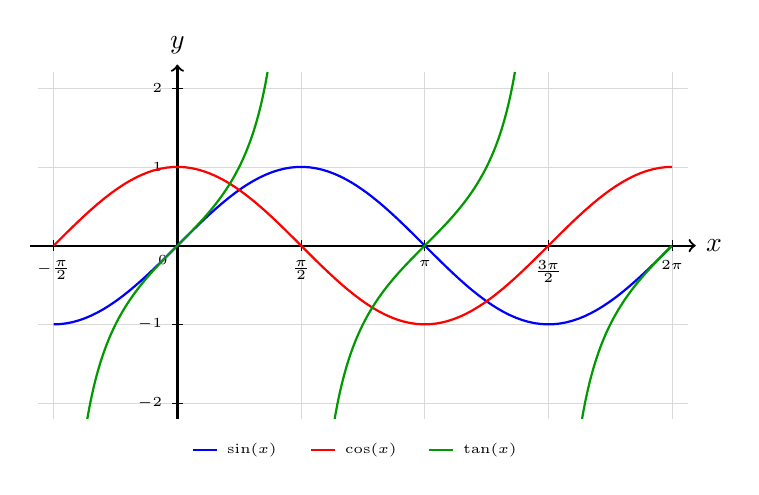
\begin{tikzpicture}
    \draw[very thin, gray!30, xstep={pi/2}, ystep=1] ({-pi/2 - 0.2}, -2.2) grid ({2*pi + 0.2}, 2.2);

    \draw[->, thick] ({-pi/2 - 0.3}, 0) -- ({2*pi + 0.3}, 0) node[right] {$x$};
    \draw[->, thick] (0, -2.2) -- (0, 2.3) node[above] {$y$};

    \draw ({-pi/2}, 2pt) -- ({-pi/2}, -2pt) node[below, font=\tiny] {$-\frac{\pi}{2}$};
    \draw ({pi/2}, 2pt)  -- ({pi/2}, -2pt)  node[below, font=\tiny] {$\frac{\pi}{2}$};
    \draw ({pi}, 2pt)    -- ({pi}, -2pt)    node[below, font=\tiny] {$\pi$};
    \draw ({3*pi/2}, 2pt)-- ({3*pi/2}, -2pt)node[below, font=\tiny] {$\frac{3\pi}{2}$};
    \draw ({2*pi}, 2pt)  -- ({2*pi}, -2pt)  node[below, font=\tiny] {$2\pi$};

    \foreach \y in {-2, -1, 1, 2}
        \draw (2pt, \y) -- (-2pt, \y) node[left, font=\tiny] {$\y$};
    \node[below left, font=\tiny] at (0,0) {$0$};

    \begin{scope}
        \clip ({-pi/2 - 0.2}, -2.2) rectangle ({2*pi + 0.1}, 2.2);

        \draw[thick, blue, domain={-pi/2}:{2*pi}, samples=100] 
            plot (\x, {sin(\x r)});

        \draw[thick, red, domain={-pi/2}:{2*pi}, samples=100] 
            plot (\x, {cos(\x r)});

        \draw[thick, green!60!black, domain=-1.4:1.4, samples=100] 
            plot (\x, {tan(\x r)});
        \draw[thick, green!60!black, domain=1.75:4.55, samples=100] 
            plot (\x, {tan(\x r)});
        \draw[thick, green!60!black, domain=4.9:6.28, samples=50] 
            plot (\x, {tan(\x r)});
    \end{scope}

    \begin{scope}[shift={(0.2, -2.6)}, font=\tiny]
        \draw[thick, blue] (0,0) -- (0.3,0) node[right, black] {$\sin(x)$};
        \draw[thick, red] (1.5,0) -- (1.8,0) node[right, black] {$\cos(x)$};
        \draw[thick, green!60!black] (3.0,0) -- (3.3,0) node[right, black] {$\tan(x)$};
    \end{scope}
\end{tikzpicture}
\end{center}
Wie man aus dem bild sehen kann, haben wir:
\begin{itemize}
    \item $\sin: \RR \to [-1, 1]$, $\forall k \in \ZZ : \sin(k\pi) = 0$
    \item $\cos: \RR \to [-1, 1]$, $\forall k \in \ZZ : \cos(k\pi + \frac{pi}{2})) = 0$
    \item $\tan: \RR\setminus\{\frac{2k + 1}{2}\pi \,|\, k \in \ZZ\} \to \RR$
\end{itemize}
\end{minipage}

\begin{minipage}{\linewidth}
\Bild Graphen von Trigonometrischen Inversen

\begin{center}
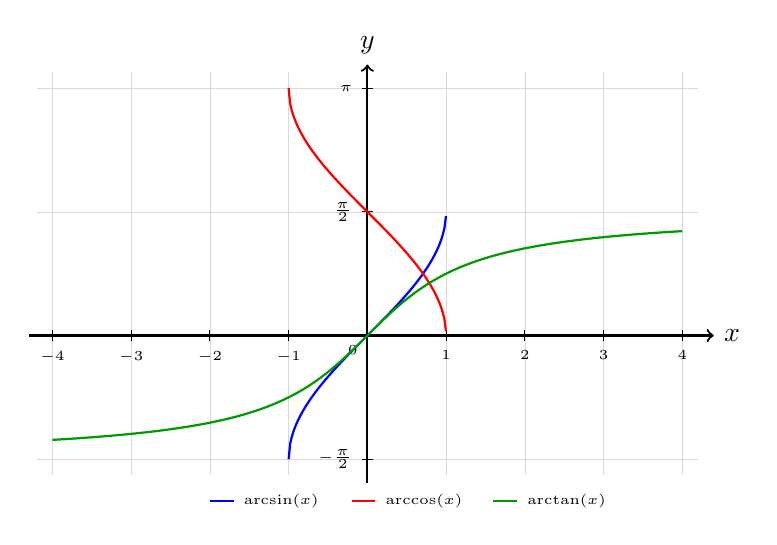
\begin{tikzpicture}
    \draw[very thin, gray!30, xstep=1, ystep={pi/2}] (-4.2, {-pi/2 - 0.2}) grid (4.2, {pi + 0.2});

    \draw[->, thick] (-4.3, 0) -- (4.4, 0) node[right] {$x$};
    \draw[->, thick] (0, {-pi/2 - 0.3}) -- (0, {pi + 0.3}) node[above] {$y$};

    \foreach \x in {-4, -3, -2, -1, 1, 2, 3, 4}
        \draw (\x, 2pt) -- (\x, -2pt) node[below, font=\tiny] {$\x$};

    \draw (2pt, {-pi/2}) -- (-2pt, {-pi/2}) node[left, font=\tiny] {$-\frac{\pi}{2}$};
    \draw (2pt, {pi/2})  -- (-2pt, {pi/2})  node[left, font=\tiny] {$\frac{\pi}{2}$};
    \draw (2pt, {pi})    -- (-2pt, {pi})    node[left, font=\tiny] {$\pi$};
    \node[below left, font=\tiny] at (0,0) {$0$};

    \begin{scope}
        \clip (-4.2, {-pi/2 - 0.2}) rectangle (4.2, {pi + 0.2});

        \draw[thick, blue, domain=-1:1, samples=100] 
            plot (\x, {rad(asin(\x))});

        \draw[thick, red, domain=-1:1, samples=100] 
            plot (\x, {rad(acos(\x))});

        \draw[thick, green!60!black, domain=-4:4, samples=100] 
            plot (\x, {rad(atan(\x))});
    \end{scope}

    \begin{scope}[shift={(-2.0, -2.1)}, font=\tiny]
        \draw[thick, blue] (0,0) -- (0.3,0) node[right, black] {$\arcsin(x)$};
        \draw[thick, red] (1.8,0) -- (2.1,0) node[right, black] {$\arccos(x)$};
        \draw[thick, green!60!black] (3.6,0) -- (3.9,0) node[right, black] {$\arctan(x)$};
    \end{scope}
\end{tikzpicture}
\end{center}
Wie man aus dem bild sehen kann, haben wir:
\begin{itemize}
    \item $\arcsin: [-1, 1] \to [-\frac{\pi}{2}, \frac{\pi}{2}]$
    \item $\arccos: [-1, 1] \to [0, \pi]$
    \item $\arctan: \RR \to (-\frac{\pi}{2}, \frac{\pi}{2})$, $\lim\limits_{x\to \pm\infty} \arctan x = \pm \frac{\pi}{2}$
\end{itemize}

\Bild Graphen von Exponentialfunktionen (und $\frac{1}{x}$ just because)

\begin{center}
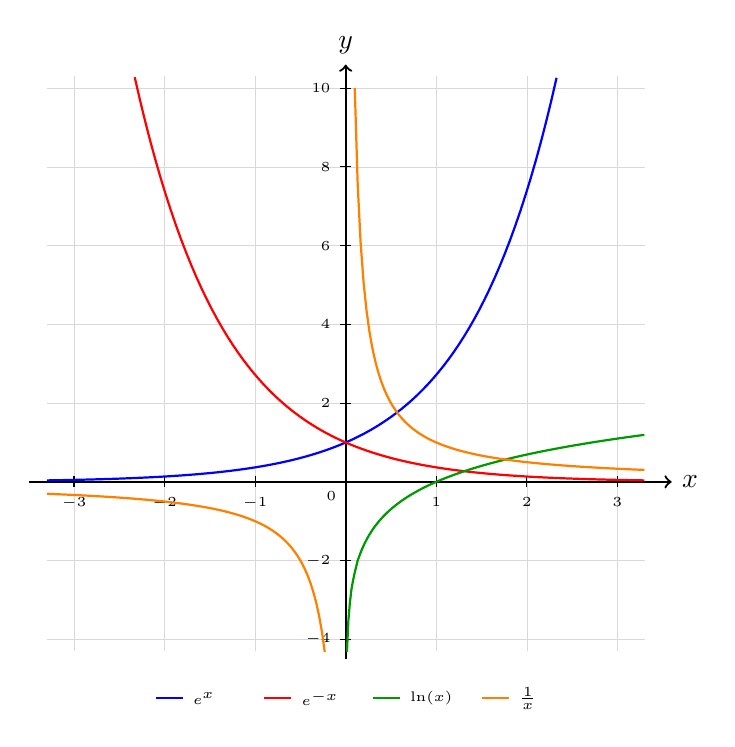
\begin{tikzpicture}[x=1.15cm, y=0.5cm]
    % Grid matching xstep = 1 and ystep = 2
    \draw[very thin, gray!30, xstep=1, ystep=2] (-3.3, -4.3) grid (3.3, 10.3);

    % Axes
    \draw[->, thick] (-3.5, 0) -- (3.6, 0) node[right] {$x$};
    \draw[->, thick] (0, -4.5) -- (0, 10.6) node[above] {$y$};

    % X-Axis Ticks (Steps of 1 from -3 to 3)
    \foreach \x in {-3, -2, -1, 1, 2, 3}
        \draw (\x, 2pt) -- (\x, -2pt) node[below, font=\tiny] {$\x$};

    % Y-Axis Ticks (Steps of 2 from -4 to 10)
    \foreach \y in {-4, -2, 2, 4, 6, 8, 10}
        \draw (2pt, \y) -- (-2pt, \y) node[left, font=\tiny] {$\y$};
    \node[below left, font=\tiny] at (0,0) {$0$};

    % Clip plot region
    \begin{scope}
        \clip (-3.3, -4.3) rectangle (3.3, 10.3);

        % 1. e^x (Blue)
        \draw[thick, blue, domain=-3.3:2.33, samples=100] 
            plot (\x, {exp(\x)});

        % 2. e^-x (Red)
        \draw[thick, red, domain=-2.33:3.3, samples=100] 
            plot (\x, {exp(-\x)});

        % 3. ln(x) (Green)
        \draw[thick, green!60!black, domain=0.013:3.3, samples=200] 
            plot (\x, {ln(\x)});

        % 4. 1/x (Orange) - Split domain to avoid x = 0 asymptote
        \draw[thick, orange, domain=-3.3:-0.1, samples=100] 
            plot (\x, {1/\x});
        \draw[thick, orange, domain=0.1:3.3, samples=100] 
            plot (\x, {1/\x});
    \end{scope}

    % Legend
    \begin{scope}[shift={(0.0, -5.5)}, font=\tiny]
        \draw[thick, blue] (-2.1,0) -- (-1.8,0) node[right, black] {$e^x$};
        \draw[thick, red] (-0.9,0) -- (-0.6,0) node[right, black] {$e^{-x}$};
        \draw[thick, green!60!black] (0.3,0) -- (0.6,0) node[right, black] {$\ln(x)$};
        \draw[thick, orange] (1.5,0) -- (1.8,0) node[right, black] {$\frac{1}{x}$};
    \end{scope}

\end{tikzpicture}
\end{center}
Wie man aus dem bild sehen kann, haben wir:
\begin{itemize}
    \item $e^x: \RR \to (0, \infty)$, $\lim\limits_{x\to -\infty} e^x = 0$, $\lim\limits_{x\to \infty} e^x = \infty$
    \item $e^{-x}: \RR \to (0, \infty)$, $\lim\limits_{x\to -\infty} e^{-x} = \infty$, $\lim\limits_{x\to \infty} e^{-x} = 0$
    \item $\ln: (0, \infty) \to \RR$, $\lim\limits_{x\to 0} \ln x = -\infty$, $\lim\limits_{x\to \infty} \ln x = \infty$
    \item $\frac{1}{x}: (-\infty, 0) \cup (0, \infty) \to \RR\setminus\{0\}$, $\lim\limits_{x\to \pm \infty} \frac{1}{x} = 0$, $\lim\limits_{x\to 0^\pm} \ln x = \pm\infty$
\end{itemize}
\end{minipage}

\begin{minipage}{\linewidth}
\Tab Wichtige Grenzwerte

\begin{tabular}{l c r}
    $\lim f(x)$ & Grenzwert $L$ & Bedingung \\
    \hline
    $\lim\limits_{n\to\infty} \frac{\ln n}{n}$ & $0$ & \\[1ex]
    $\lim\limits_{n\to\infty} \sqrt[n]{n}$ & $1$ & \\[1ex]
    $\lim\limits_{n\to\infty} \sqrt[n]{x}$ & $1$ & $x > 0$ \\[1ex]
    $\lim\limits_{n\to\infty} \left(1 + \frac{x}{n}\right)^n$ & $e^x$ & $x \in \mathbb{R}$ \\[1ex]
    $\lim\limits_{n\to\infty} \frac{x^n}{n!}$ & $0$ & $x \in \mathbb{R}$ \\[0.5ex]
    \hline
    $\lim\limits_{n\to\infty} x^n$ & $0$ & $|x| < 1$ \\[1ex]
    $\lim\limits_{n\to\infty} \frac{n^k}{a^n}$ & $0$ & $a > 1, k \in \mathbb{R}$ \\[1ex]
    $\lim\limits_{n\to\infty} \frac{a^n}{n!}$ & $0$ & $a > 0$ \\[1ex]
    $\lim\limits_{n\to\infty} \frac{n!}{n^n}$ & $0$ & \\[1ex]
    $\lim\limits_{n\to\infty} \sqrt[n]{a^n + b^n}$ & $\max(a, b)$ & $a, b \ge 0$ \\
    \hline
    $\lim\limits_{x\to 0} \frac{\sin x}{x}$ & $1$ & $x \neq 0$ \\[1ex]
    $\lim\limits_{x\to 0} \frac{\sin (ax)}{x}$ & $a$ & $x \neq 0, a \in \RR$ \\[1ex]
    $\lim\limits_{x\to 0} \frac{1 - \cos x}{x^2}$ & $\frac{1}{2}$ & $x \neq 0$ \\[1ex]
    $\lim\limits_{x\to 0} \frac{e^x - 1}{x} = \lim\limits_{x\to 0} \frac{e^x}{x + 1}$ & $1$ & $x \neq 0$ \\[1ex]
    $\lim\limits_{x\to 0} \frac{\ln(1 + x)}{x}$ & $1$ & $x > -1, x \neq 0$ \\[1ex]
    $\lim\limits_{x\to 0} \frac{(1 + x)^k - 1}{x}$ & $k$ & $k \in \mathbb{R}, x \neq 0$ \\[0.5ex]
    \hline
    $\lim\limits_{x\to 0^+} x^x$ & $1$ & \\[1ex]
    $\lim\limits_{x\to 0^+} x^a \ln x$ & $0$ & $a > 0$ \\[1ex]
    $\lim\limits_{x\to\infty} \frac{(\ln x)^k}{x^a}$ & $0$ & $a > 0, k \in \mathbb{R}$
\end{tabular}
\end{minipage}

\begin{minipage}{\linewidth}
\Tab Wichtige Maclaurin-Reihen

\begin{tabular}{l c c r}
    $f(x)$ & Entwicklung & Summenform & Bedingung \\
    \hline
    $e^x$ & $1 + x + \frac{x^2}{2!} + \dots$ & $\sum_{k=0}^\infty \frac{x^k}{k!}$ & $x \in \mathbb{R}$ \\[1ex]
    $\cos x$ & $1 - \frac{x^2}{2!} + \frac{x^4}{4!} - \dots$ & $\sum_{k=0}^\infty (-1)^k \frac{x^{2k}}{(2k)!}$ & $x \in \mathbb{R}$ \\[1ex]
    $\sin x$ & $x - \frac{x^3}{3!} + \frac{x^5}{5!} - \dots$ & $\sum_{k=0}^\infty (-1)^k \frac{x^{2k+1}}{(2k+1)!}$ & $x \in \mathbb{R}$ \\[1ex]
    $\cosh x$ & $1 + \frac{x^2}{2!} + \frac{x^4}{4!} + \dots$ & $\sum_{k=0}^\infty \frac{x^{2k}}{(2k)!}$ & $x \in \mathbb{R}$ \\[1ex]
    $\sinh x$ & $x + \frac{x^3}{3!} + \frac{x^5}{5!} + \dots$ & $\sum_{k=0}^\infty \frac{x^{2k+1}}{(2k+1)!}$ & $x \in \mathbb{R}$ \\[1ex]
    \hline
    $\frac{1}{1-x}$ & $1 + x + x^2 + \dots$ & $\sum_{k=0}^\infty x^k$ & $|x| < 1$ \\[1ex]
    $\frac{1}{1+x}$ & $1 - x + x^2 - \dots$ & $\sum_{k=0}^\infty (-1)^k x^k$ & $|x| < 1$ \\[1ex]
    $\frac{x}{(1+x)^2}$ & $1 - x + 2x^2 - \dots$ & $\sum_{k=0}^\infty k x^k$ & $|x| < 1$ \\[1ex]
    $\ln(1+x)$ & $x - \frac{x^2}{2} + \frac{x^3}{3} + \dots$ & $\sum_{k=1}^\infty (-1)^{k-1} \frac{x^k}{k}$ & $-1 < x \le 1$ \\[1ex]
    $\arctan x$ & $x - \frac{x^3}{3} + \frac{x^5}{5} - \dots$ & $\sum_{k=0}^\infty (-1)^k \frac{x^{2k+1}}{2k+1}$ & $|x| \le 1$ \\[1ex]
    $(1+x)^\alpha$ & $1 + \alpha x + \dots$ & $\sum_{k=0}^\infty \binom{\alpha}{k} x^k$ & $|x| < 1$ \\
\end{tabular}
\end{minipage}

\begin{minipage}{\linewidth}
\Tab Ableitungen und Stammfunktionen

\begin{tabular}{l c r}
    $f(x)$ & $f'(x)$ & $\int f(x) \, dx (+ C)$ \\
    \hline
    $x^n \ (n \neq -1)$ & $n x^{n-1}$ & $\frac{x^{n+1}}{n+1}$ \\[1ex]
    $\frac{1}{x}$ & $-\frac{1}{x^2}$ & $\ln|x|$ \\[1ex]
    $e^x$ & $e^x$ & $e^x$ \\[1ex]
    $a^x$ & $a^x \ln a$ & $\frac{a^x}{\ln a}$ \\[1ex]
    $\ln x$ & $\frac{1}{x}$ & $x \ln x - x$ \\[0.5ex]
    \hline
    $\sin x$ & $\cos x$ & $-\cos x$ \\[1ex]
    $\cos x$ & $-\sin x$ & $\sin x$ \\[1ex]
    $\tan x$ & $\sec^2 x$ & $-\ln|\cos x|$ \\[1ex]
    $\sec x$ & $\sec x \tan x$ & $\ln|\sec x + \tan x|$ \\[1ex]
    $\csc x$ & $-\csc x \cot x$ & $-\ln|\csc x + \cot x|$ \\[1ex]
    $\cot x$ & $-\csc^2 x$ & $\ln|\sin x|$ \\
    \hline
    $\arcsin x$ & $\frac{1}{\sqrt{1-x^2}}$ & $x \arcsin x + \sqrt{1-x^2}$ \\[1ex]
    $\arccos x$ & $-\frac{1}{\sqrt{1-x^2}}$ & $x \arccos x - \sqrt{1-x^2}$ \\[1ex]
    $\arctan x$ & $\frac{1}{1+x^2}$ & $x \arctan x - \frac{1}{2}\ln(1+x^2)$ \\[0.5ex]
    \hline
    $\sinh x$ & $\cosh x$ & $\cosh x$ \\[1ex]
    $\cosh x$ & $\sinh x$ & $\sinh x$ \\[1ex]
    $\tanh x$ & $\operatorname{sech}^2 x$ & $\ln(\cosh x)$ \\
\end{tabular}
\end{minipage}

\begin{minipage}{\linewidth}
\Tab Trigonometrische Identitäten

\begin{tabular}{l l}
    $\sin x = \cos(x - \frac{\pi}{2})$ & $\cos x = \sin(x + \frac{\pi}{2})$ \\[1ex]
    $\tan x = \dfrac{\sin x}{\cos x}$ & $\sin^2 x + \cos^2 x = 1$ \\[1ex]
    $1 + \tan^2 x = \dfrac{1}{\cos^2 x}$ & $1 + \cot^2 x = \dfrac{1}{\sin^2 x}$ \\[1.5ex]
    \hline
    $\sin(-x) = -\sin x$ & $\cos(-x) = \cos x$ \\[1ex]
    $\tan(-x) = -\tan x$ & \\[0.5ex]
    \hline
    \multicolumn{2}{l}{$\sin(x \pm y) = \sin x \cos y \pm \cos x \sin y$} \\[1ex]
    \multicolumn{2}{l}{$\cos(x \pm y) = \cos x \cos y \mp \sin x \sin y$} \\[1ex]
    \multicolumn{2}{l}{$\tan(x \pm y) = \dfrac{\tan x \pm \tan y}{1 \mp \tan x \tan y}$} \\[0.5ex]
    \hline
    $\sin(2x) = 2\sin x \cos x$ & $\tan(2x) = \dfrac{2\tan x}{1 - \tan^2 x}$ \\[1ex]
    \multicolumn{2}{l}{$\cos(2x) = \cos^2 x - \sin^2 x = 2\cos^2 x - 1 = 1 - 2\sin^2 x$} \\[1ex]
    $\sin^2 x = \dfrac{1 - \cos(2x)}{2}$ & $\cos^2 x = \dfrac{1 + \cos(2x)}{2}$ \\[1ex]
    \hline
    \multicolumn{2}{l}{$\sin x + \sin y = 2 \sin\!\left(\frac{x+y}{2}\right)\cos\!\left(\frac{x-y}{2}\right)$} \\[1ex]
    \multicolumn{2}{l}{$\sin x - \sin y = 2 \cos\!\left(\frac{x+y}{2}\right)\sin\!\left(\frac{x-y}{2}\right)$} \\[1ex]
    \multicolumn{2}{l}{$\cos x + \cos y = 2 \cos\!\left(\frac{x+y}{2}\right)\cos\!\left(\frac{x-y}{2}\right)$} \\[1ex]
    \multicolumn{2}{l}{$\cos x - \cos y = -2 \sin\!\left(\frac{x+y}{2}\right)\sin\!\left(\frac{x-y}{2}\right)$} \\[1ex]
    \hline
    $\sin x \cos y = \frac{1}{2}[\sin(x+y) + \sin(x-y)]$ & \\[1ex]
    $\cos x \cos y = \frac{1}{2}[\cos(x-y) + \cos(x+y)]$ & \\[1ex]
    $\sin x \sin y = \frac{1}{2}[\cos(x-y) - \cos(x+y)]$ & \\[0.5ex]
    \hline
    $\cosh^2 x - \sinh^2 x = 1$ & $\sinh(2x) = 2\sinh x \cosh x$ \\[1ex]
    $\cosh(2x) = \cosh^2 x + \sinh^2 x$ & $e^{ix} = \cos x + i \sin x$ \\
\end{tabular}
\end{minipage}



\end{multicols*}

\pagebreak

\clearpage

\end{document}
